\subsection{The Effect of Number of Variants on SQL Generators}
\label{sec:exp-vars}


%\begin{wrapfigure}{r}{0.5\linewidth}
%\centering
%\rule{0.9\linewidth}{0.75\linewidth}
%\caption{Dummy figure.}
%\label{fig:myfig}
%\end{wrapfigure}
%\blindtext
\begin{figure}
\begin{subfigure}{.4\linewidth}
\centering
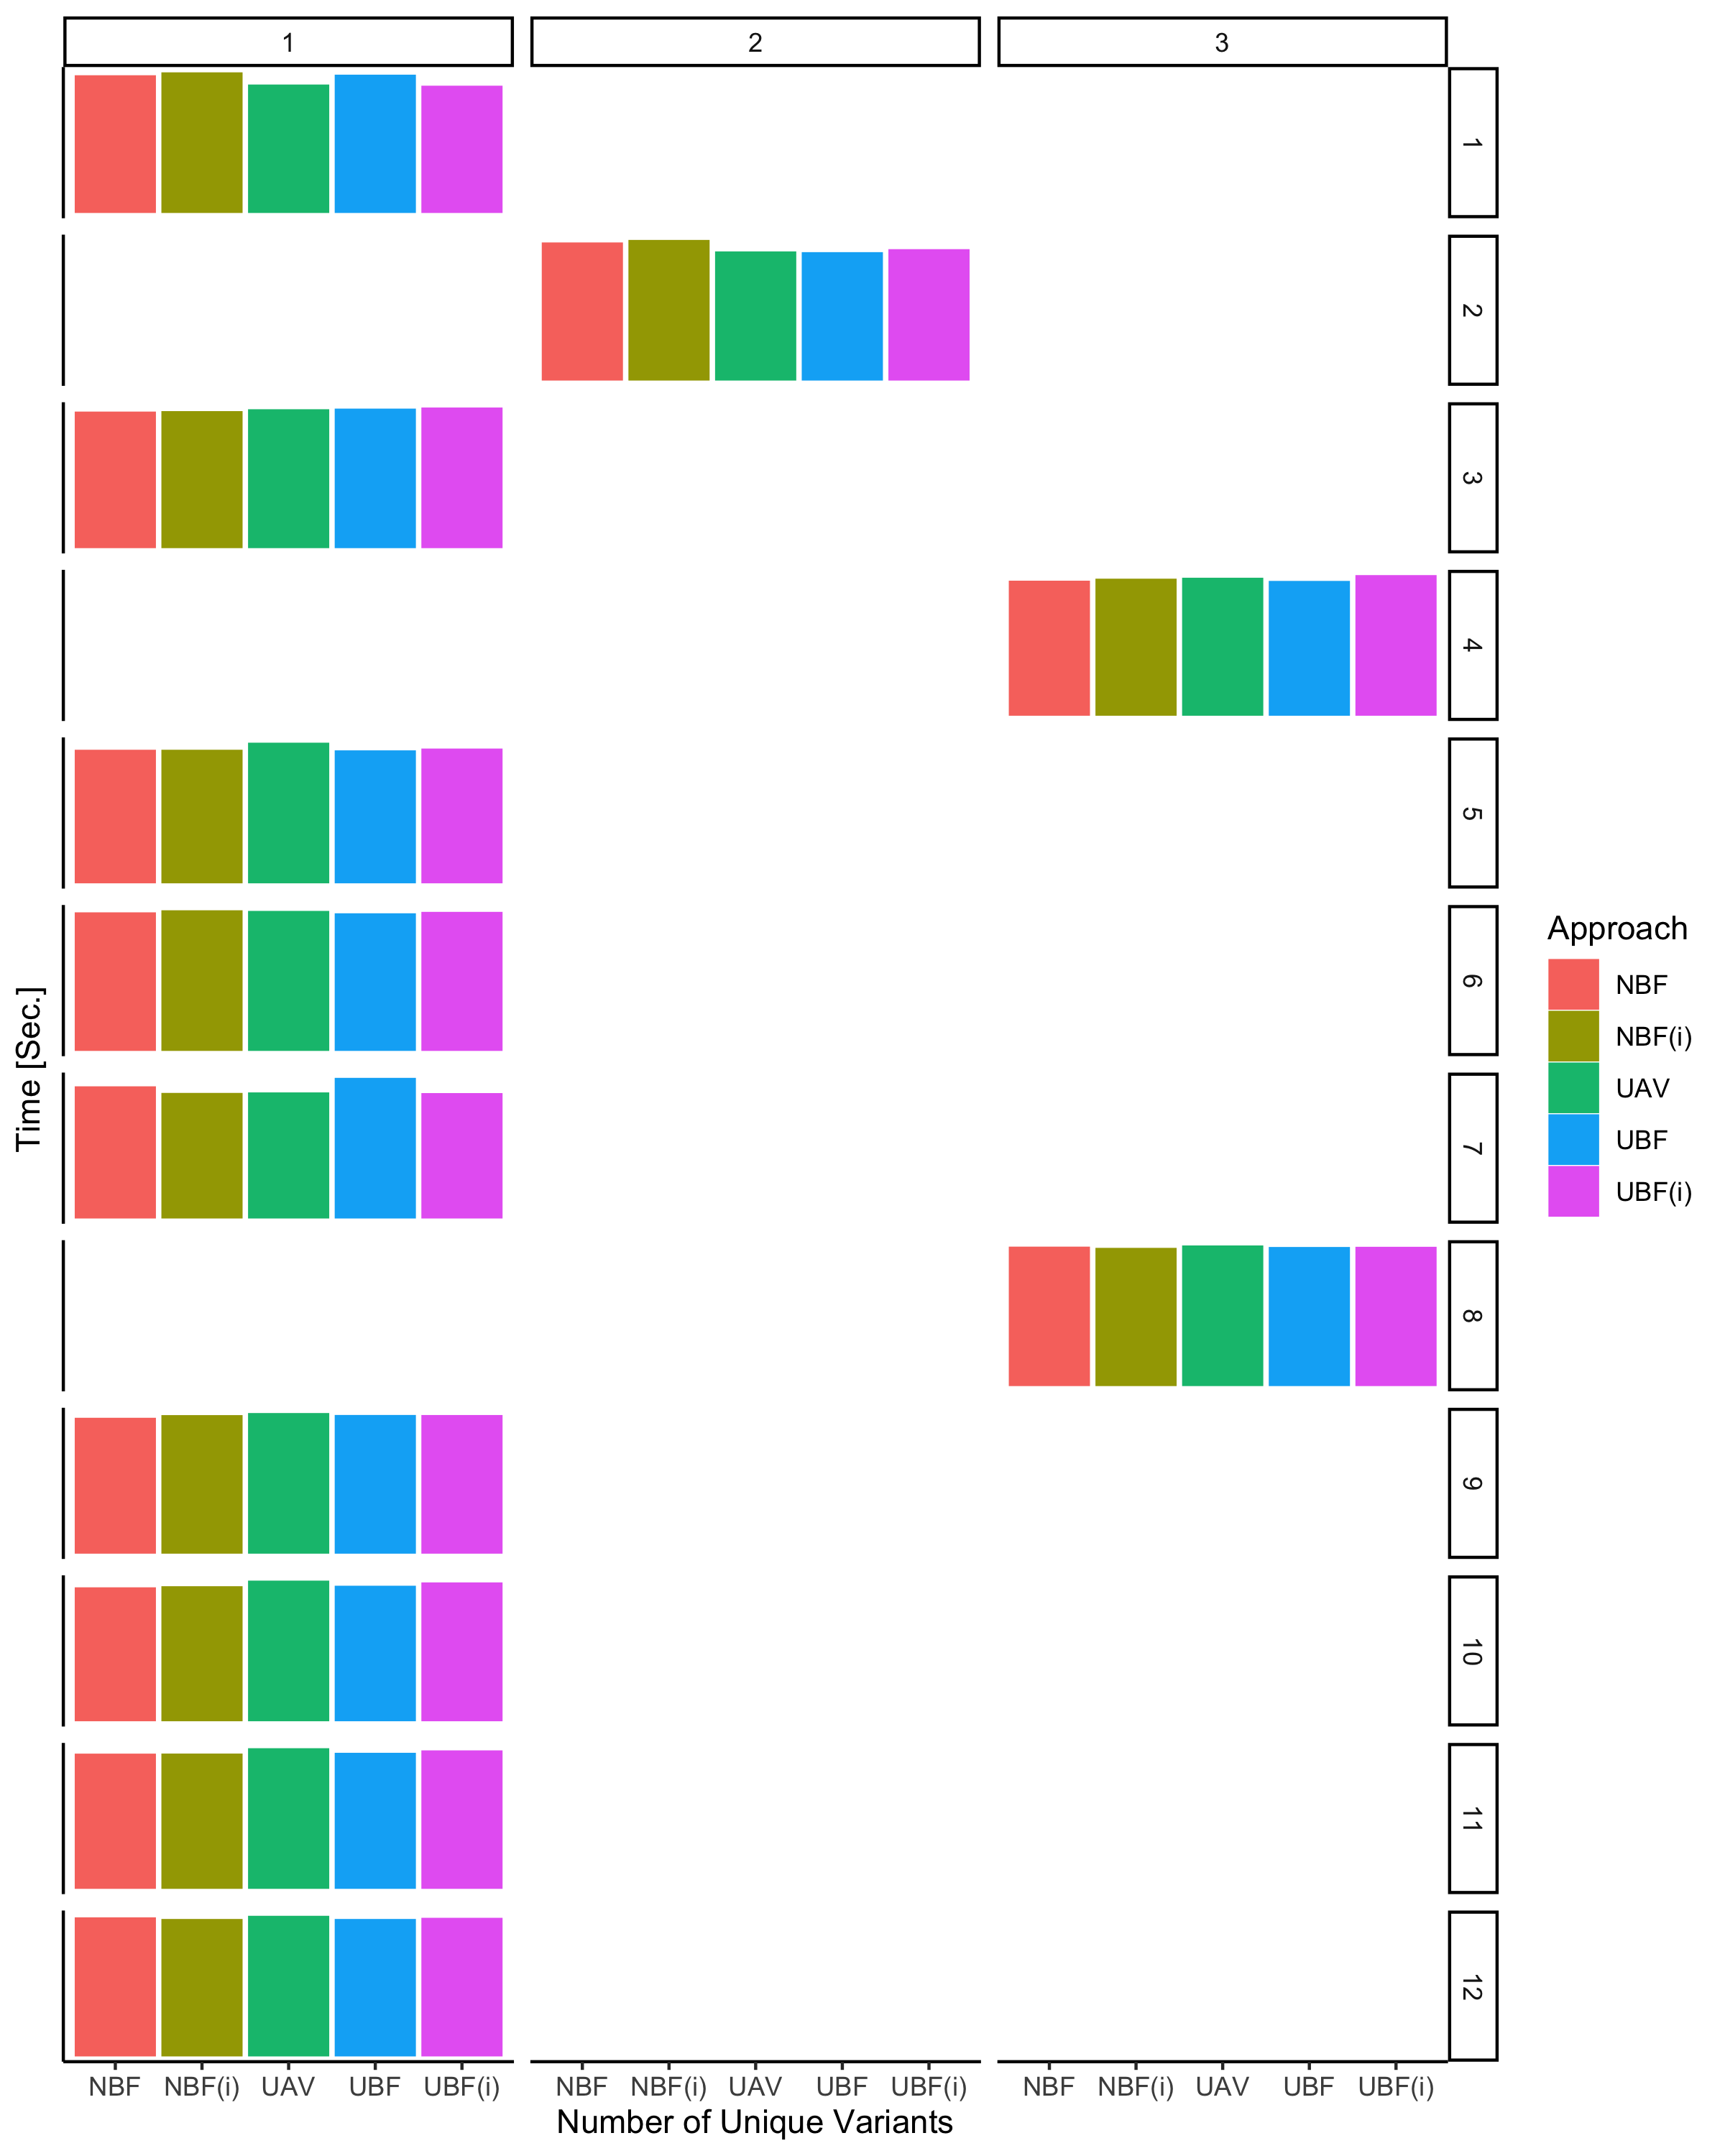
\includegraphics[width=\textwidth] {figs/plots/emp-comp-var.png}
\caption[The employee VDB]{The employee VDB.}
\label{fig:emp-var-comp}
\end{subfigure}
\begin{subfigure}{.6\linewidth}
\centering
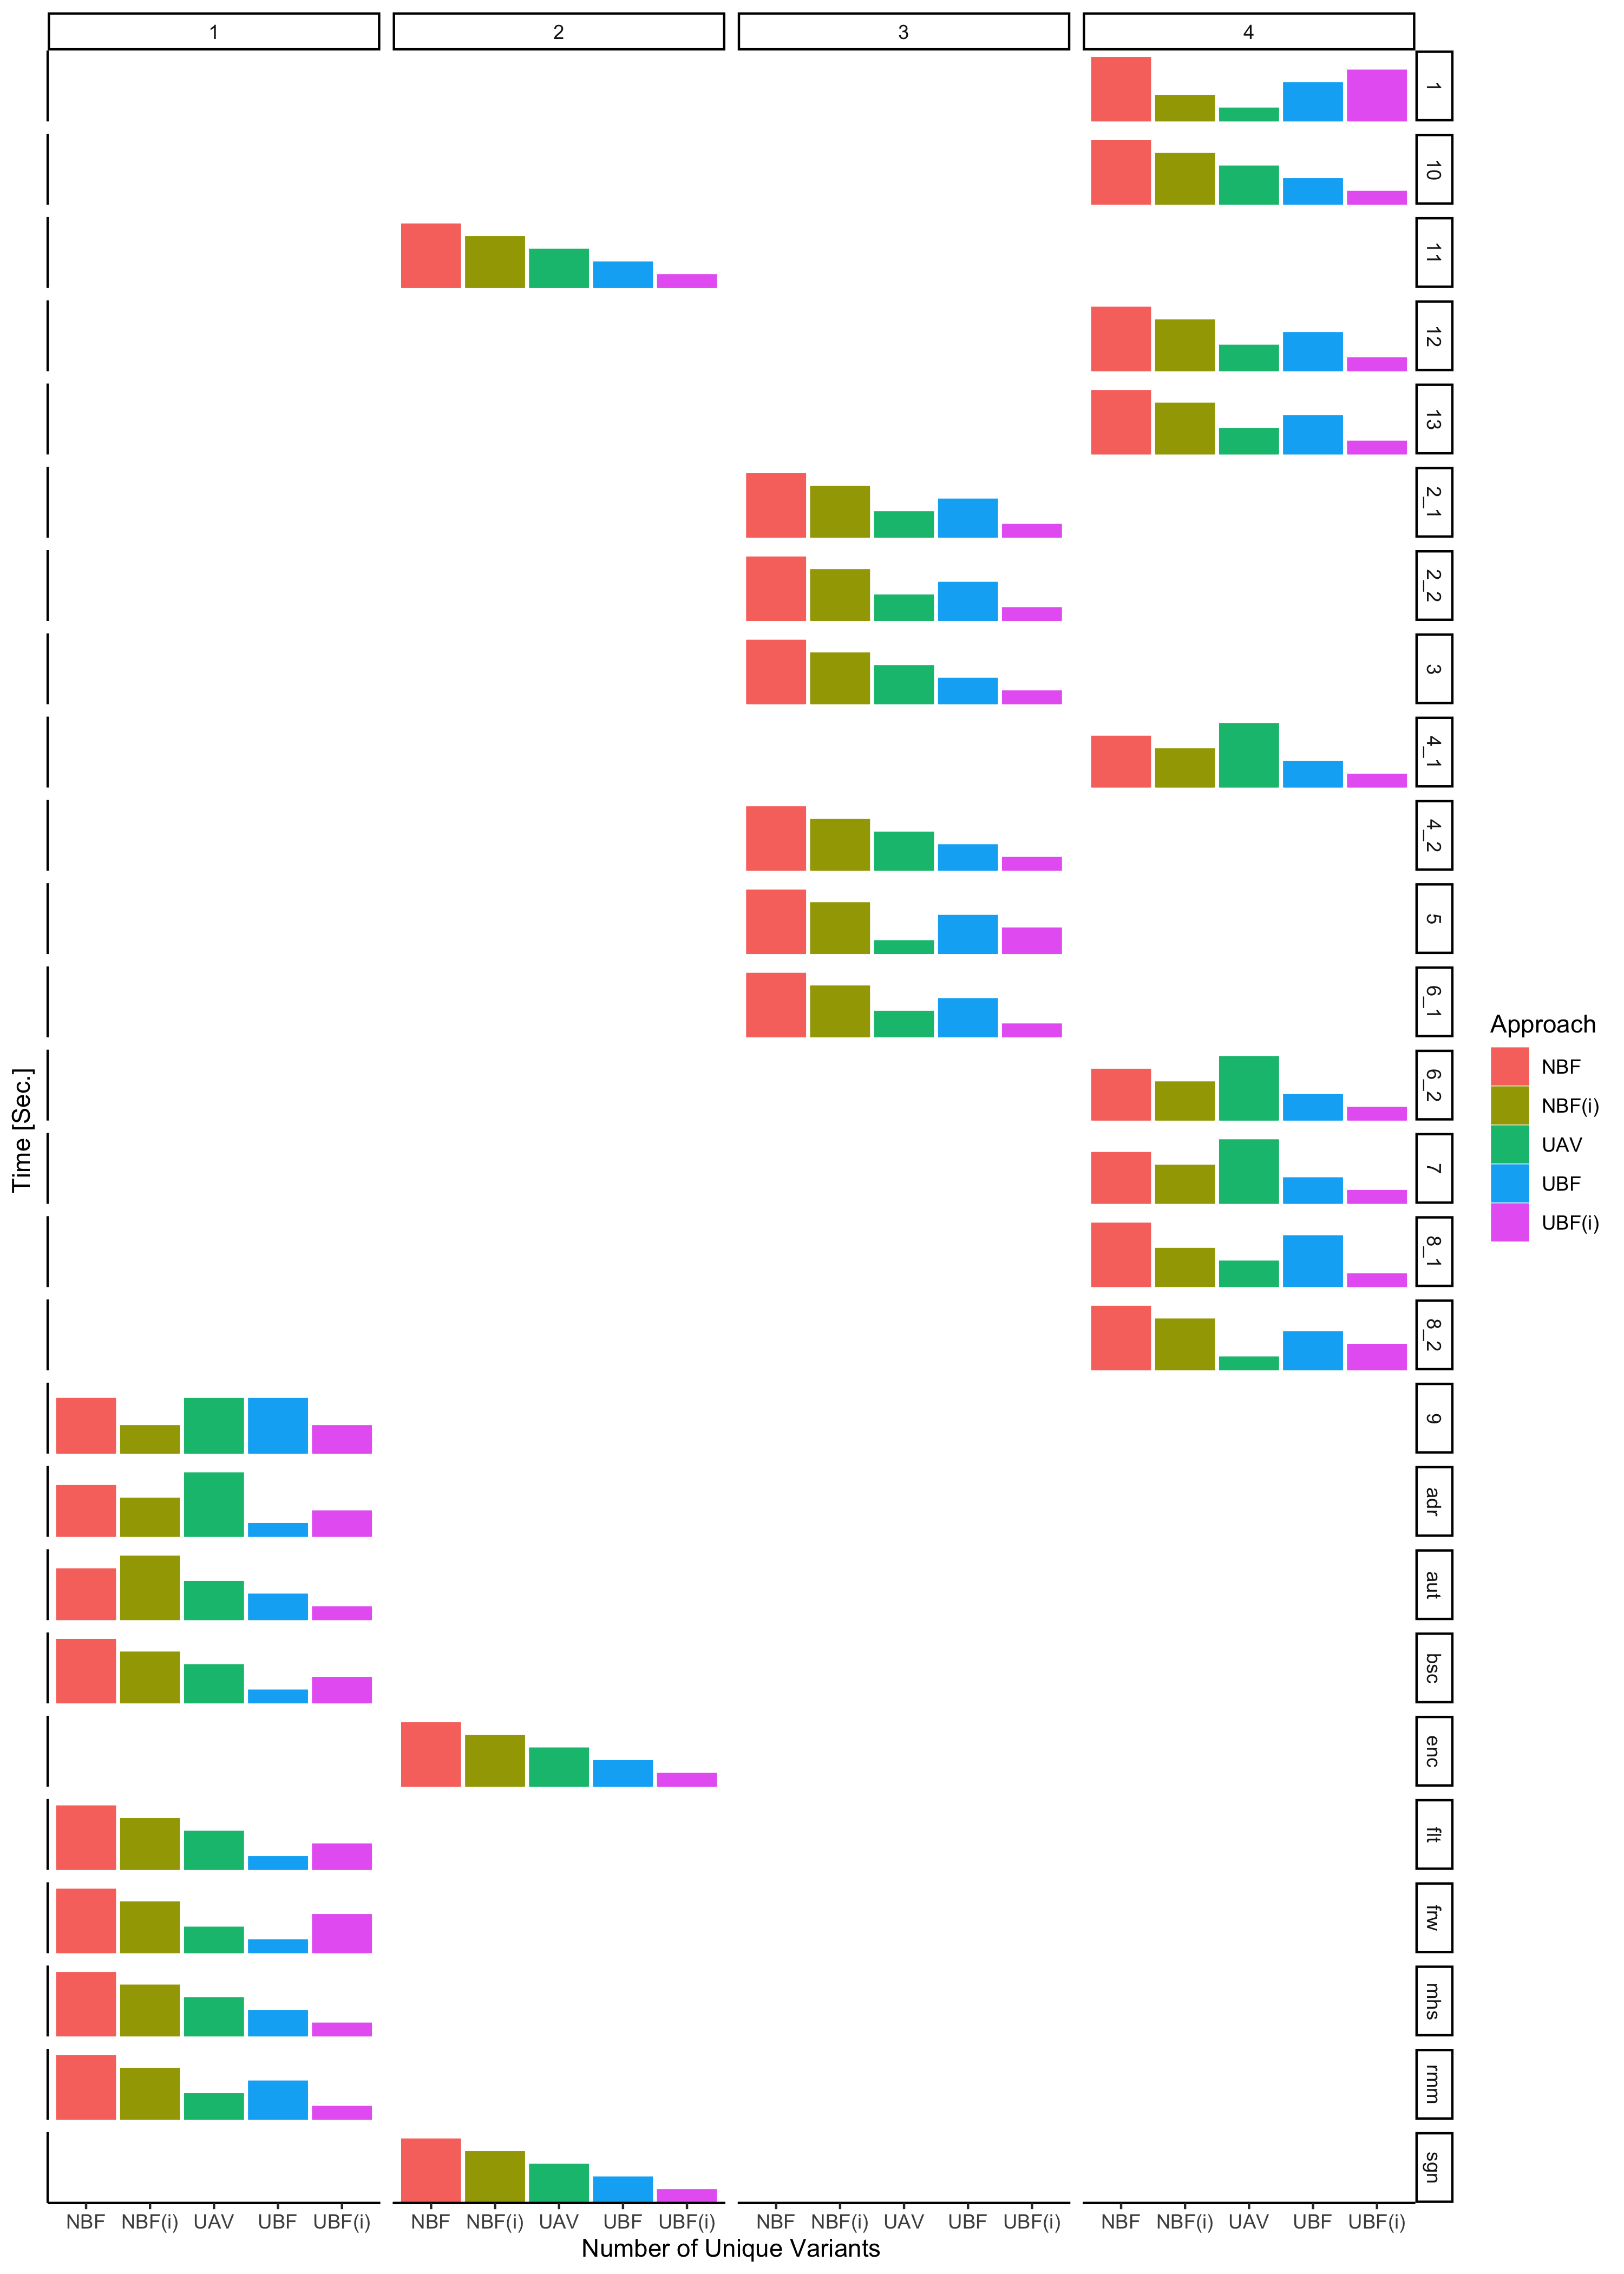
\includegraphics[width=\textwidth] {figs/plots/enron-comp-var.png}
\caption[The email VDB]{The email VDB.}
\label{fig:enron-var-comp}
\end{subfigure}
\caption[The performance of SQL generators as the number of unique variants of queries increases]{The performance of SQL generators as the number of unique variants of queries increases. The categorical boxes on the top of the plot show the number of
unique variants for each query and the categorical boxes on the right demonstrate the query 
numbers/names. Note that the striped bars indicate a N/A value due to the limitation of the
\uav\ approach explained in \secref{exp-gen}.}
\label{fig:var-comp}
\end{figure}


In this section, we explore the effect of number of variants and uniquer variants of a 
variational query on its runtime in all approaches. 
%
\figref{var-comp} illustrates the impact of the number of unique variants of variational
queries in both the employee and email VDB. 
%
The categorical boxes on top and left side of the plots indicate the number of unique
variants and the number/name of queries, respectively. 
%
\figref{emp-var-comp} does 
not provide much insight since the approaches all scale linearly with the number of unique.
However, \figref{enron-var-comp} suggests an ordering of the approaches by their performance behavior, as $\nbf \leq \nbfi \leq \ubf \leq \uav \leq \ubfi$
for most queries of this dataset. Thus, the \uav\ and \ubfi\ approaches seem to have
a better performance as the number of uniquer variants increases. 


%\begin{figure}
%\centering
%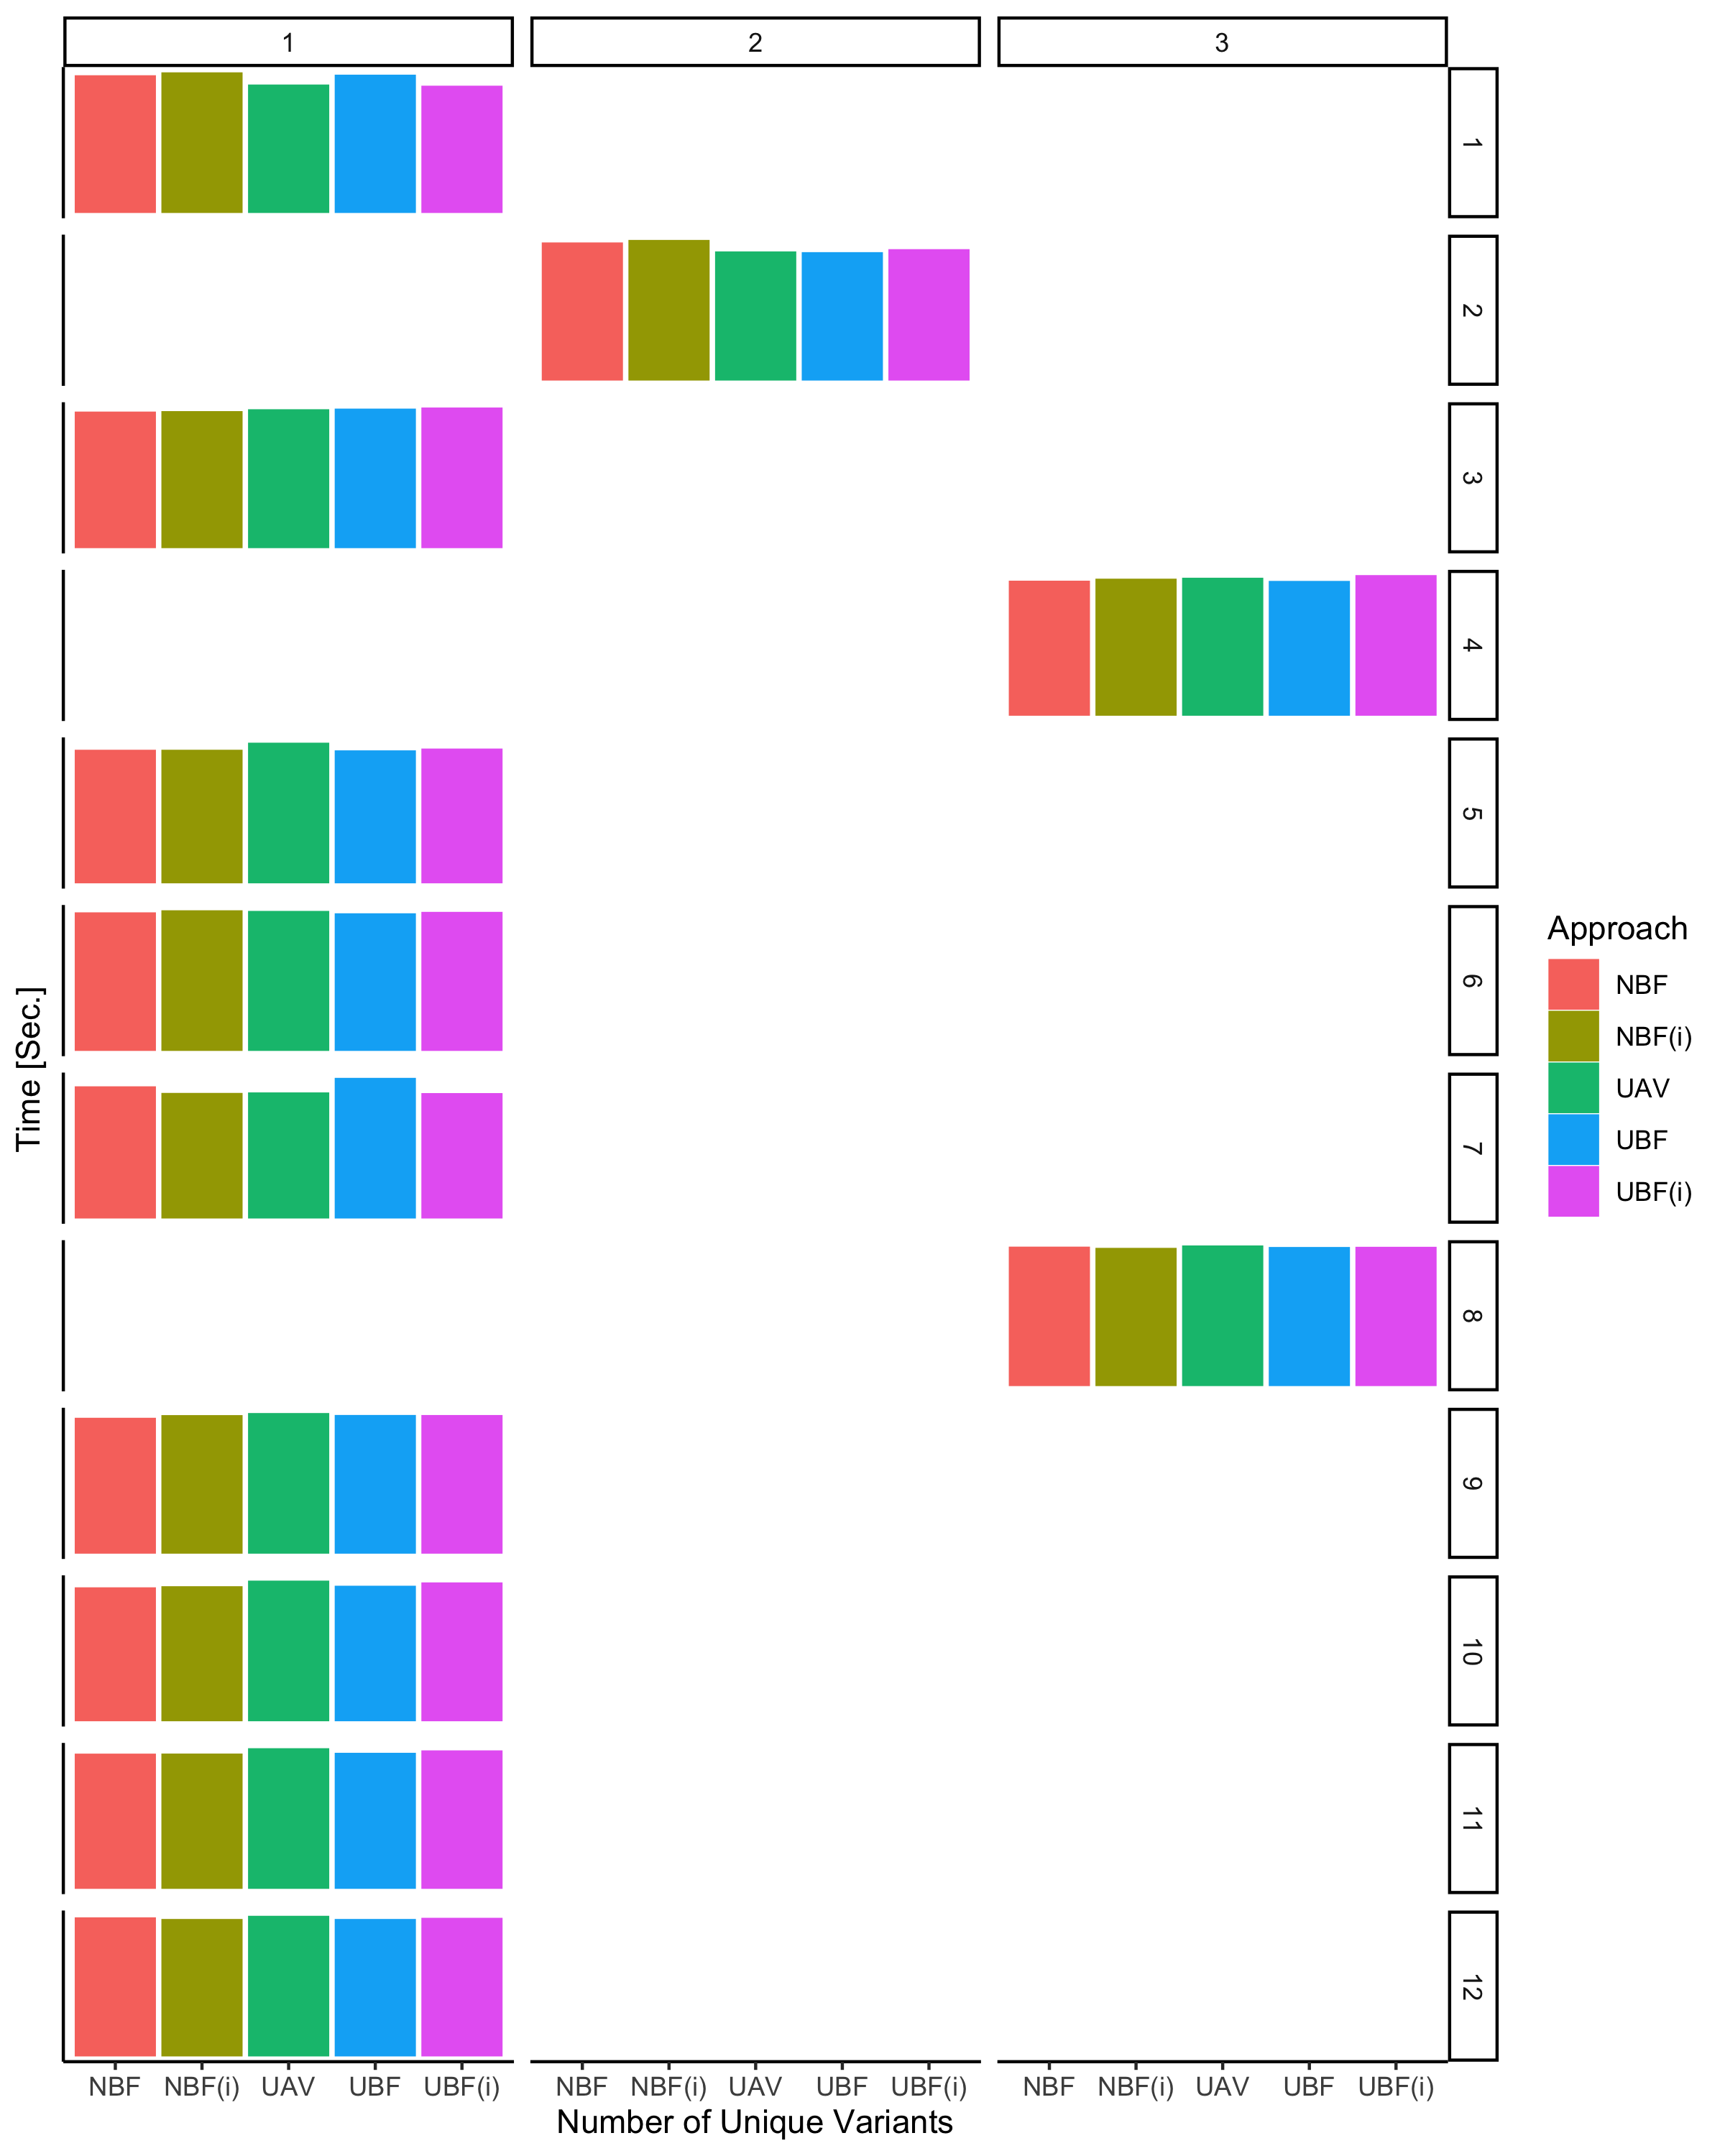
\includegraphics[scale = 0.1] {figs/plots/emp-comp-var.png}
%\caption[The performance of SQL generators as the number of unique variants of queries increases in the employee VDB]{The performance of SQL generators as the number of unique variants of queries increases in the employee VDB. The categorical boxes on top of the plot show the number of
%unique variants for each query and the categorical boxes on the right demonstrate the query 
%numbers.}
%\label{fig:emp-var-comp}
%\end{figure}
%
%\begin{figure}
%\centering
%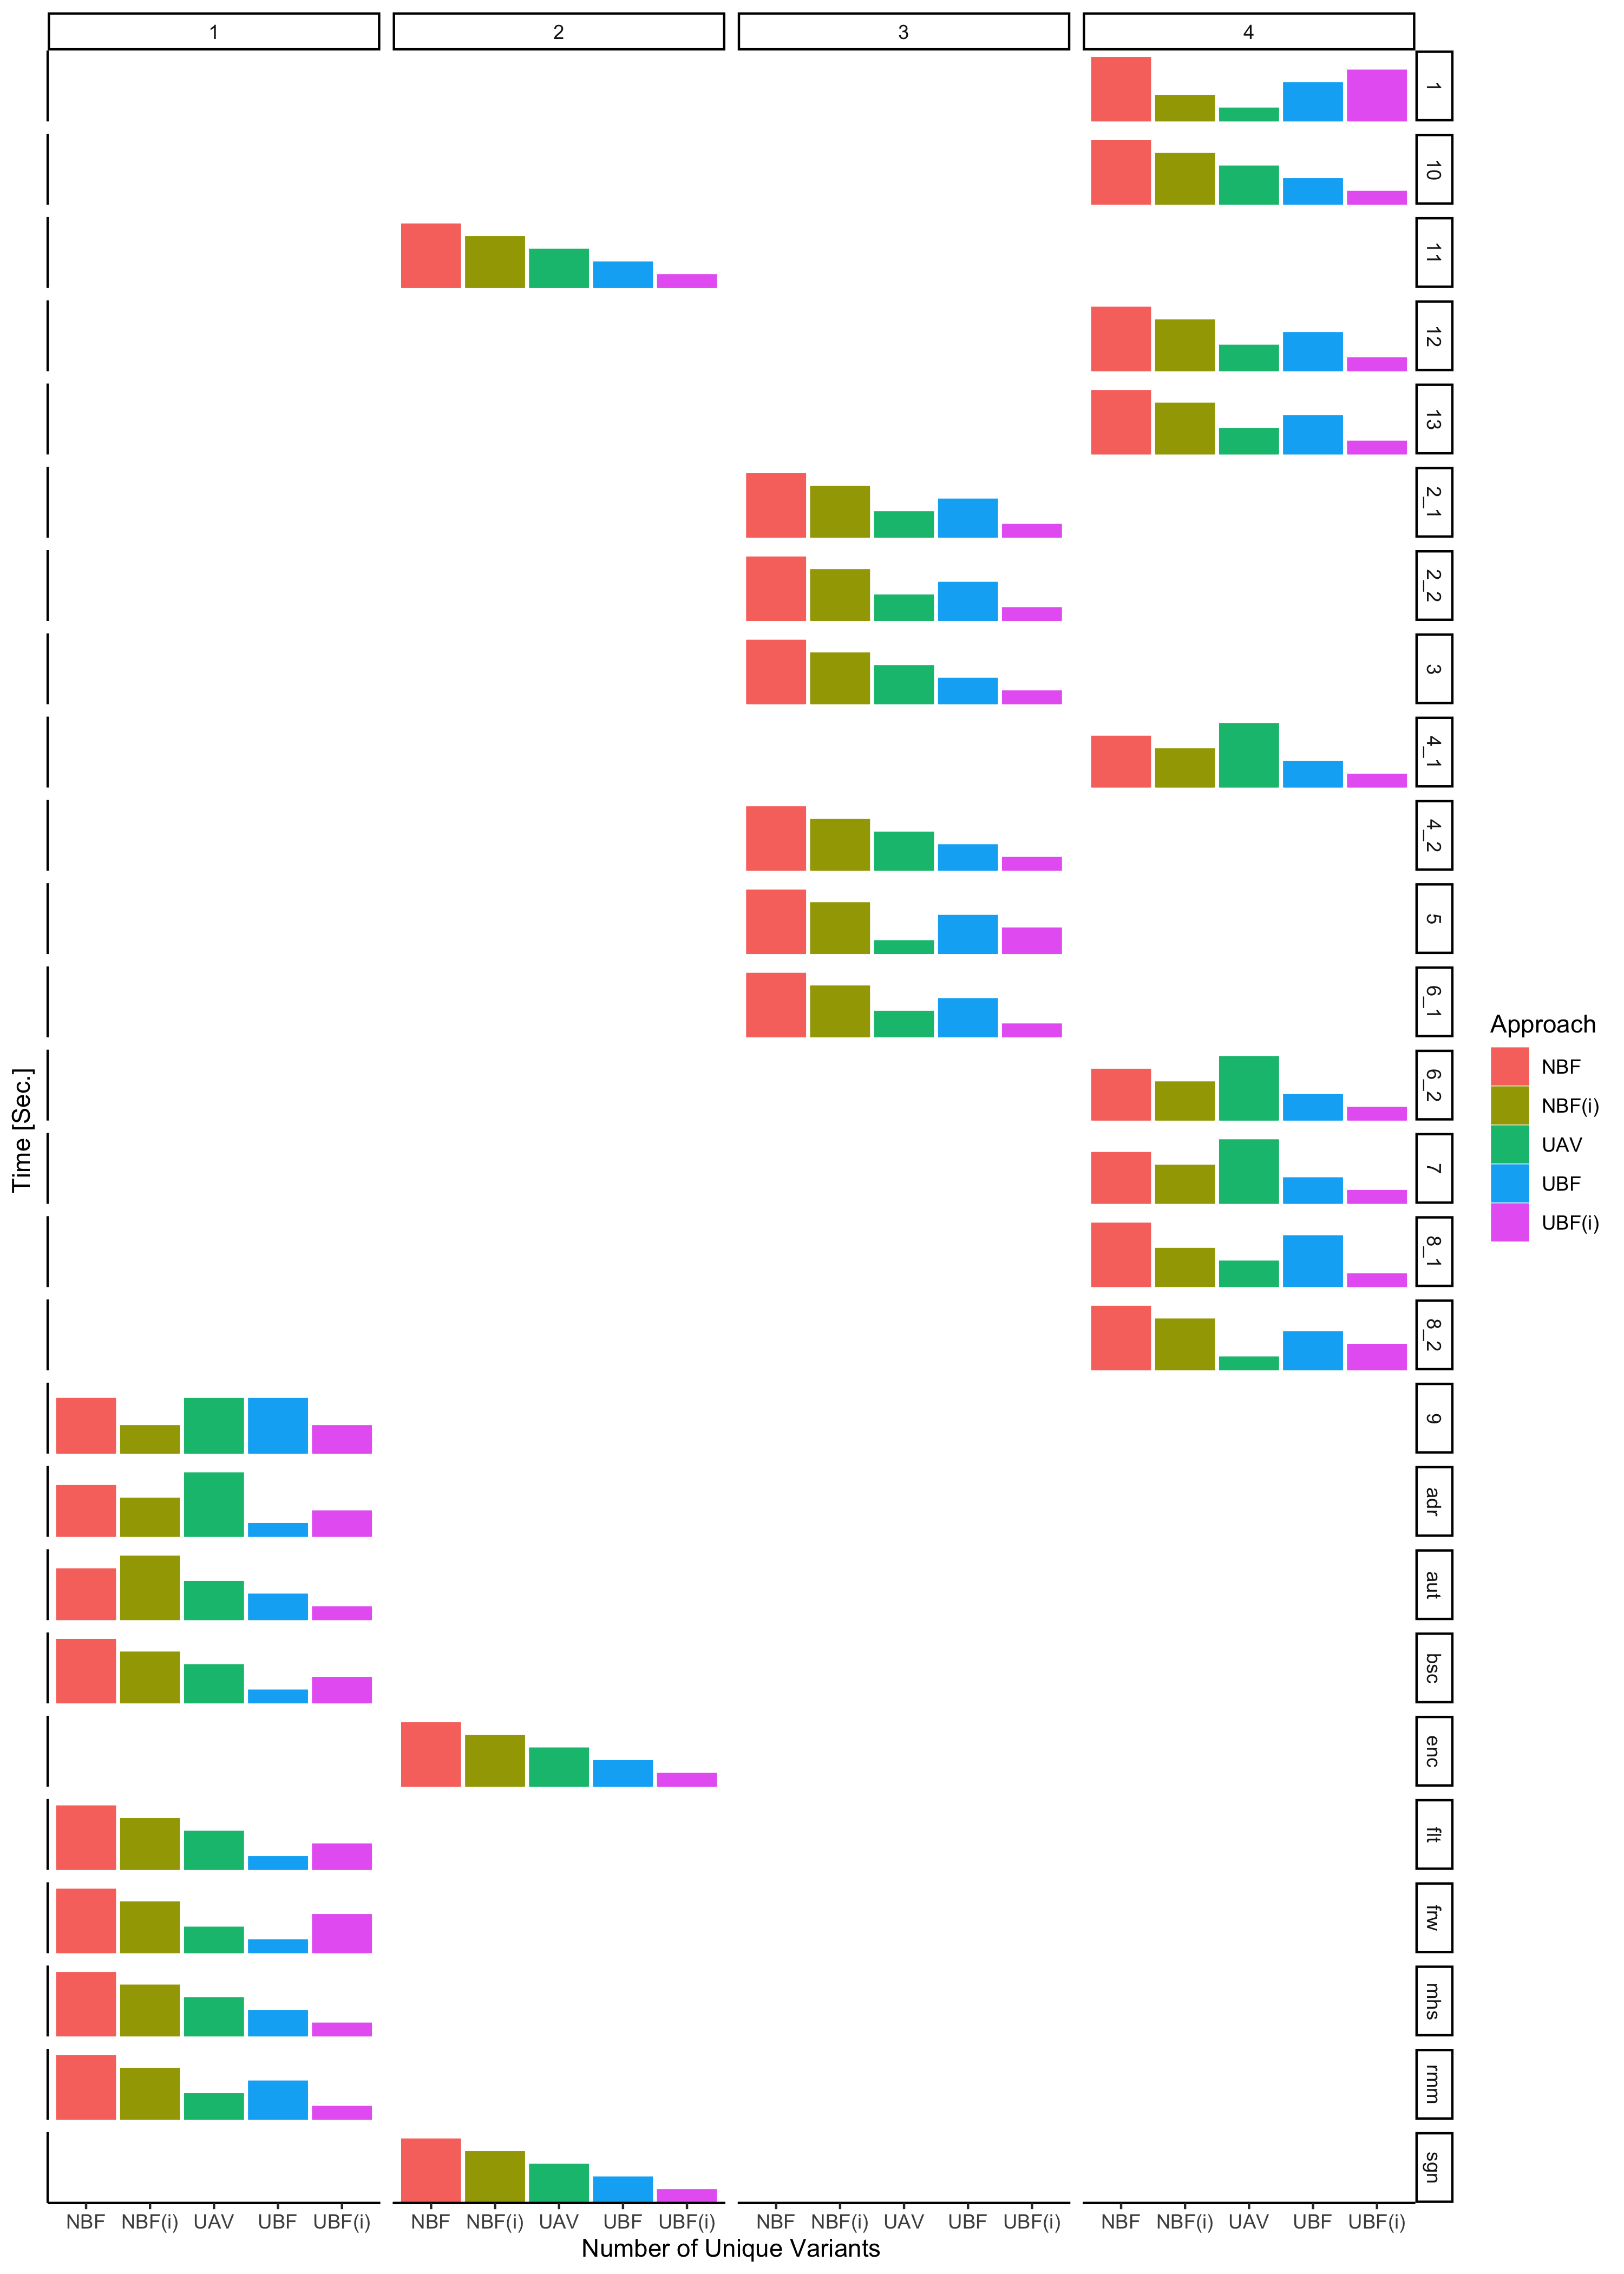
\includegraphics[scale=0.1] {figs/plots/enron-comp-var.png}
%\caption[The performance of SQL generators as the number of unique variants of queries increases in the email VDB]{The performance of SQL generators as the number of unique variants of queries increases in the email VDB. The categorical boxes on top of the plot show the number of
%unique variants for each query and the categorical boxes on the right demonstrate the query 
%numbers/names.}
%\label{fig:enron-var-comp}
%\end{figure}

\begin{figure}[!t]
\begin{subfigure}{.5\linewidth}
\centering
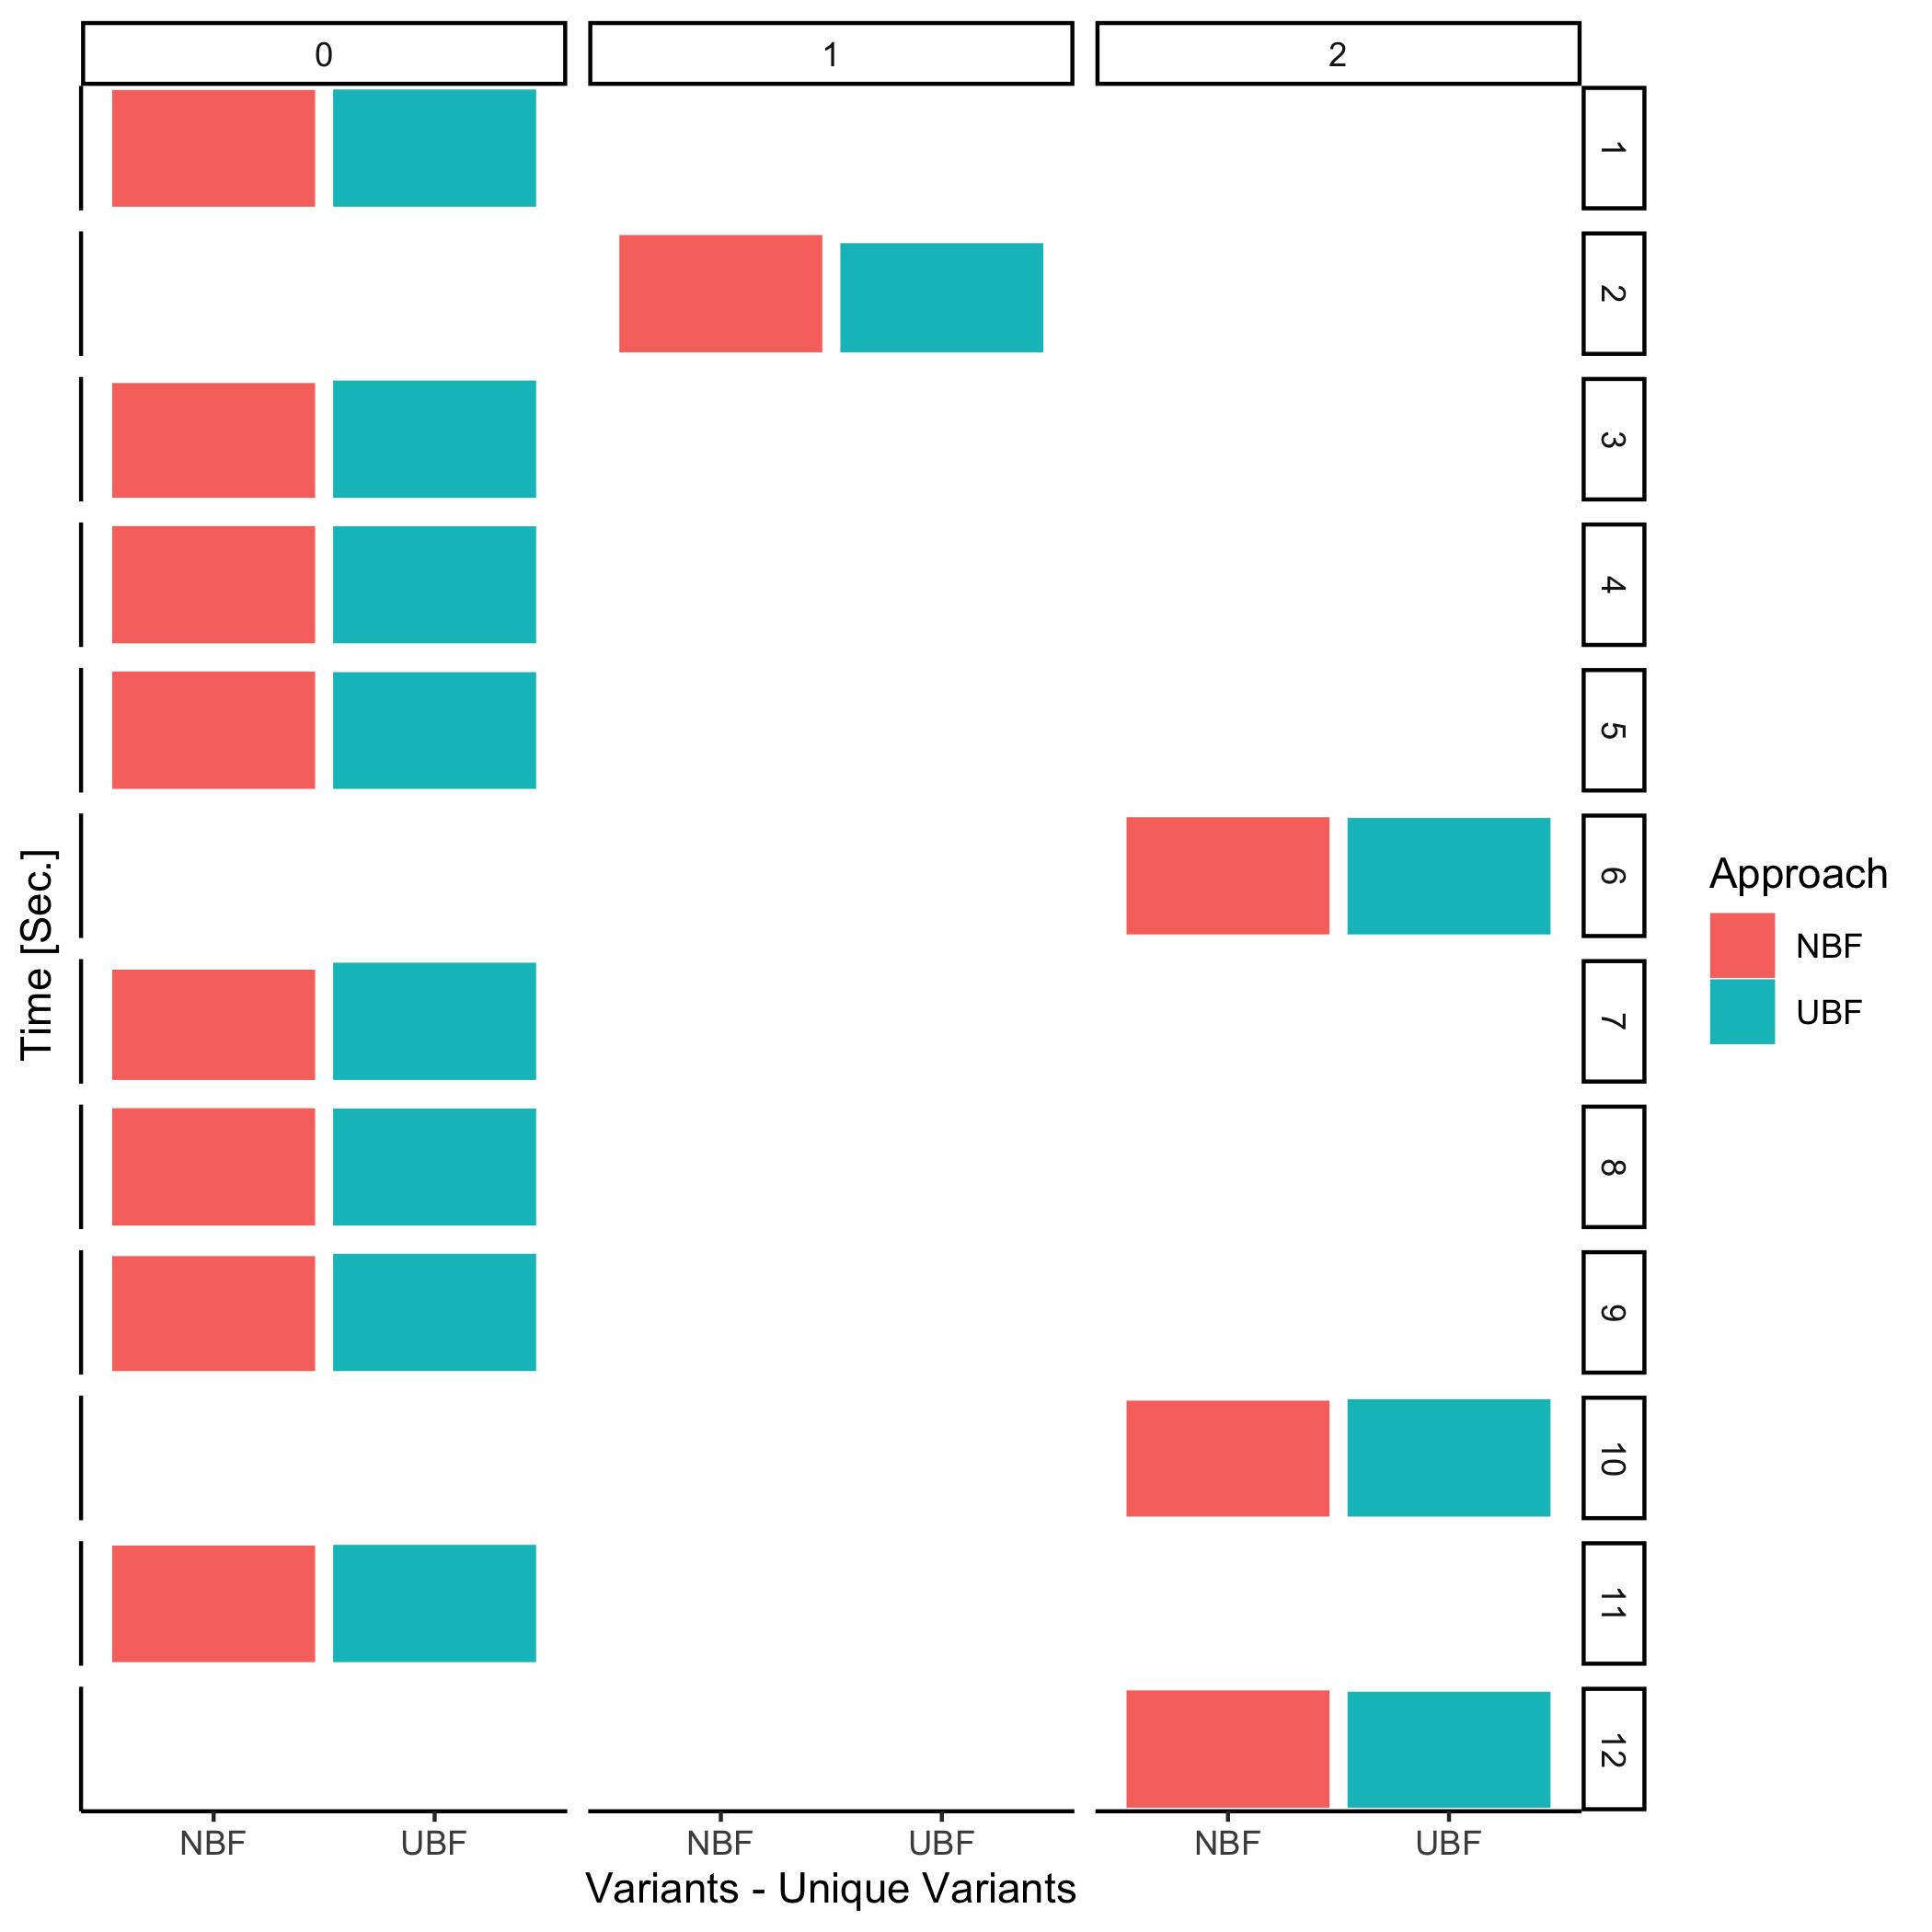
\includegraphics[width=.7\textwidth]{figs/plots/emp-nbf-ubf.png}
\caption[Comparison of the \nbf\ and \ubf\ approaches]{Comparison of the \nbf\ and \ubf\ approaches.}
\label{fig:emp-nbf-ubf}
\end{subfigure}%
\begin{subfigure}{.5\linewidth}
\centering
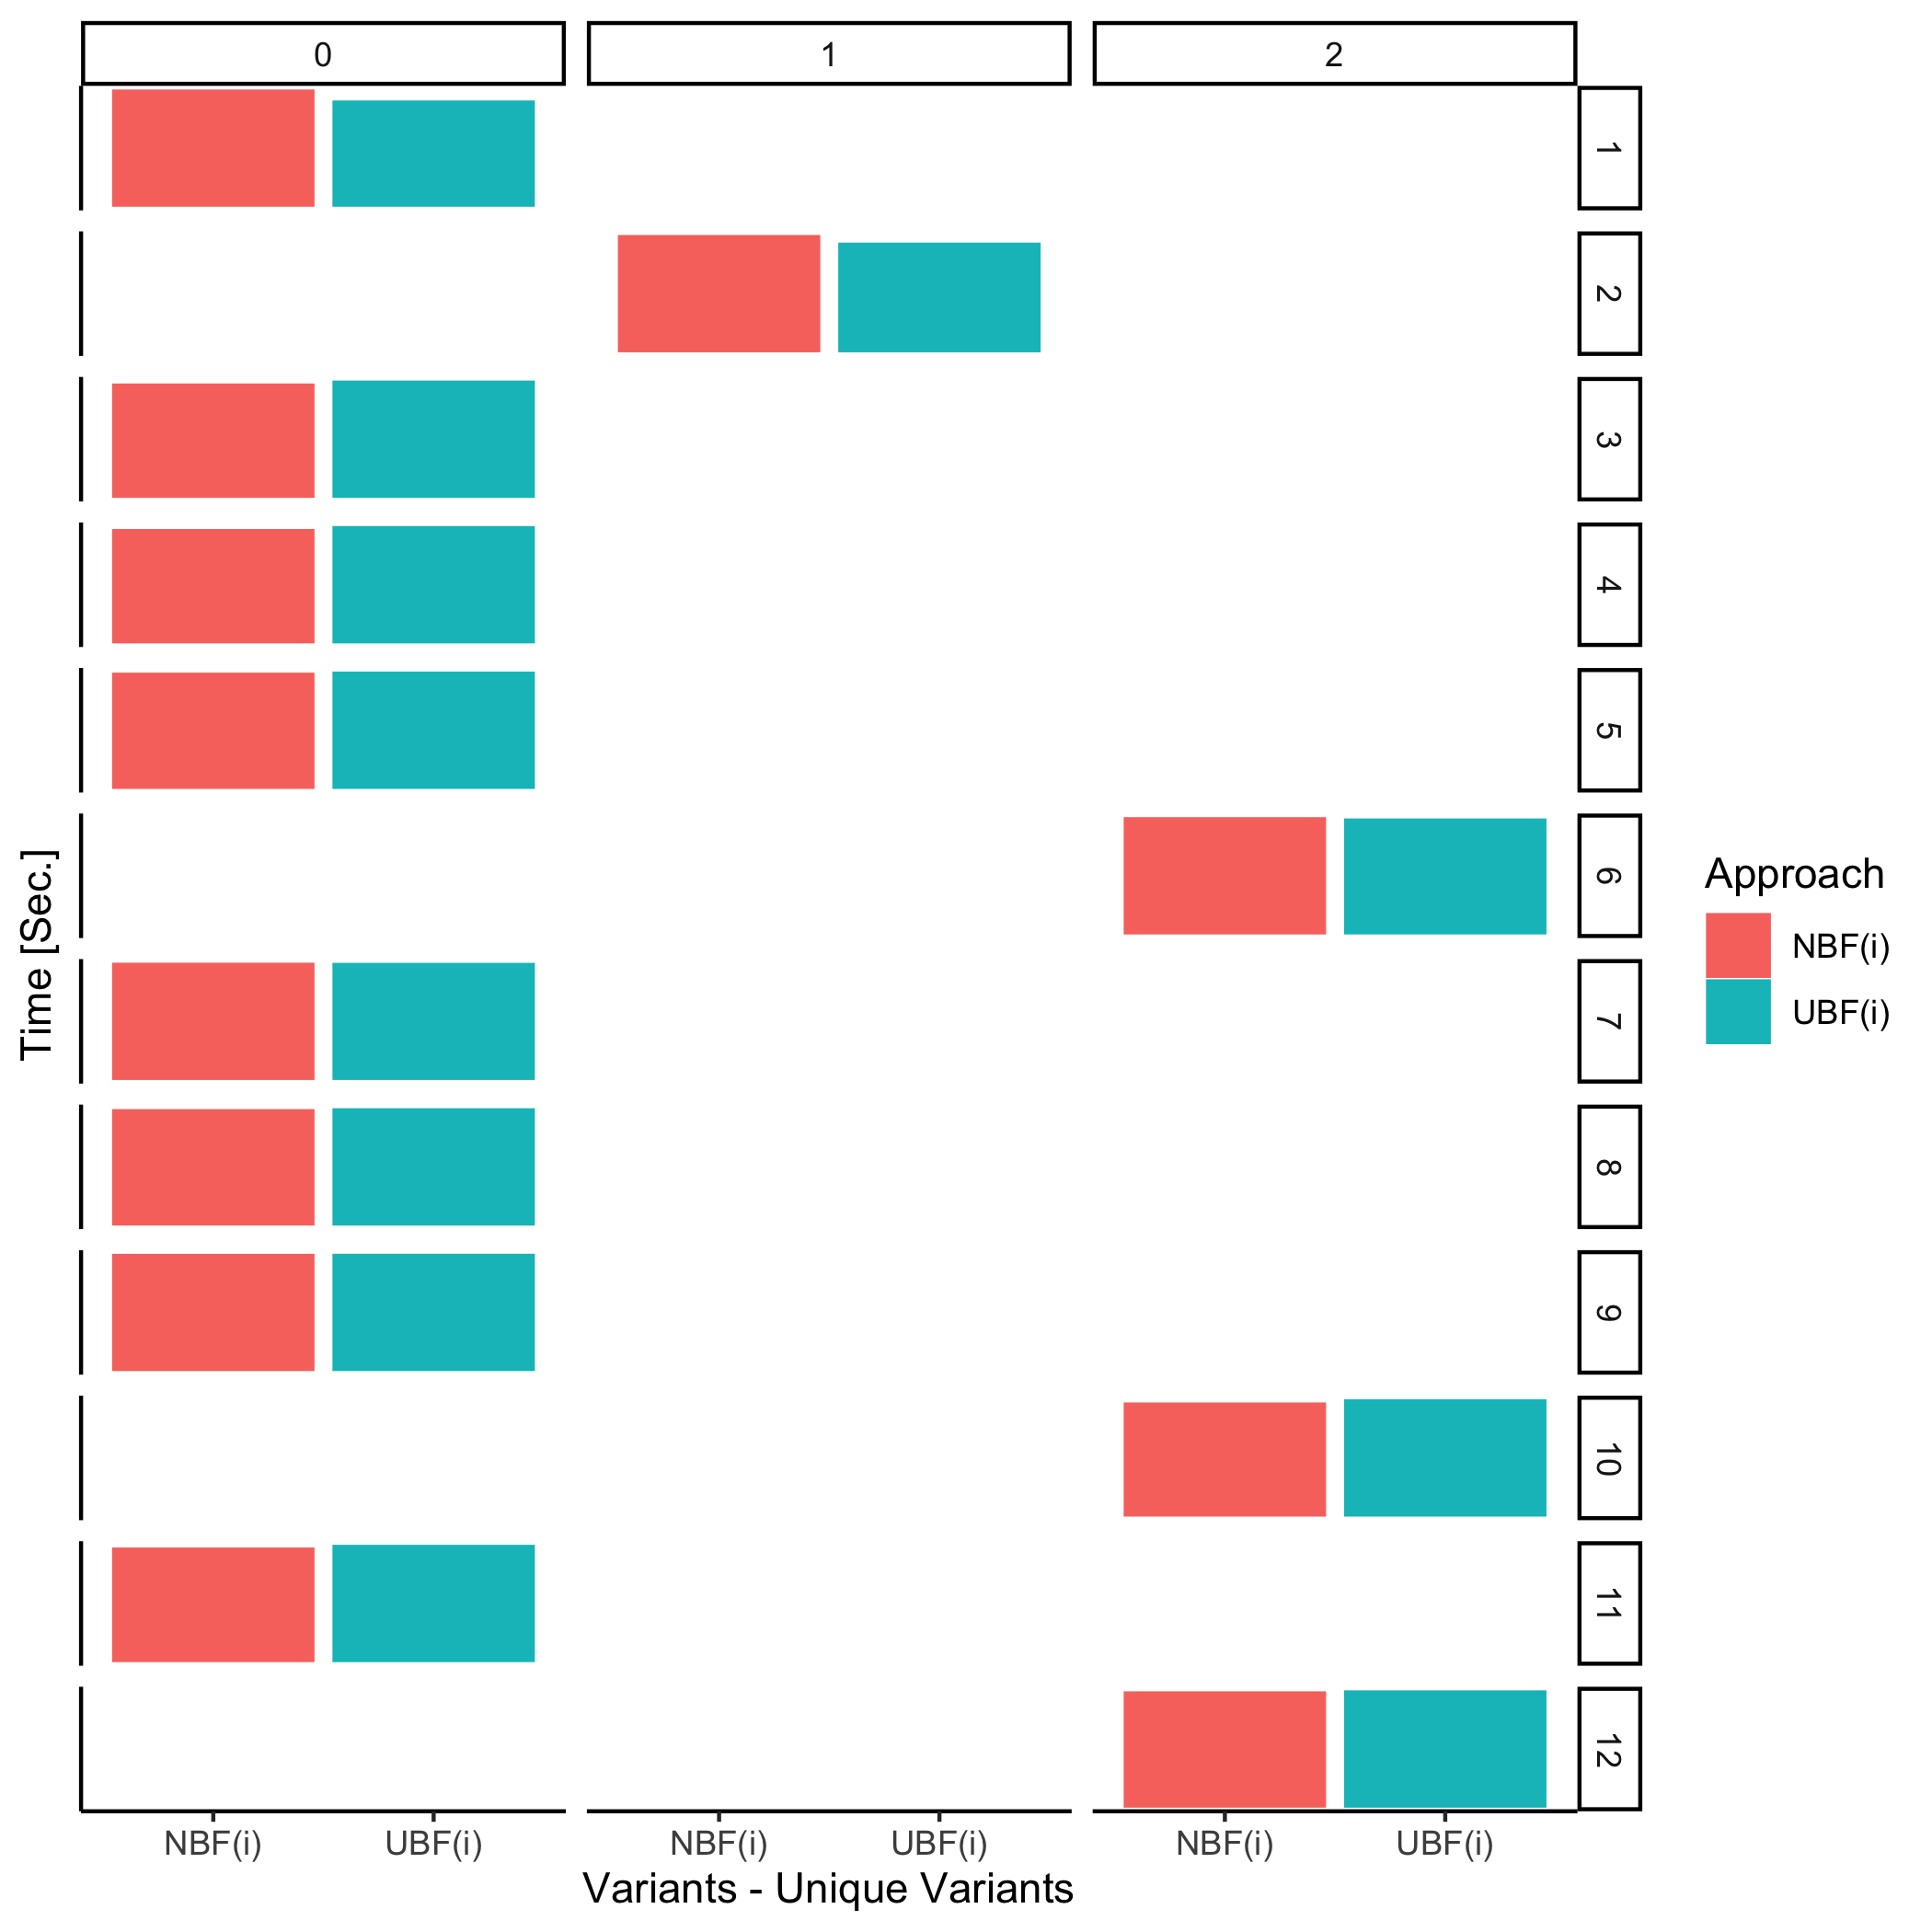
\includegraphics[width=.7\textwidth]{figs/plots/emp-nbfi-ubfi.png}
\caption[Comparison of the \nbfi\ and \ubfi\ approaches]{Comparison of the \nbfi\ and \ubfi\ approaches.}
\label{fig:emp-nbfi-ubfi}
\end{subfigure}\\[1ex]
\begin{subfigure}{0.5\linewidth}
\centering
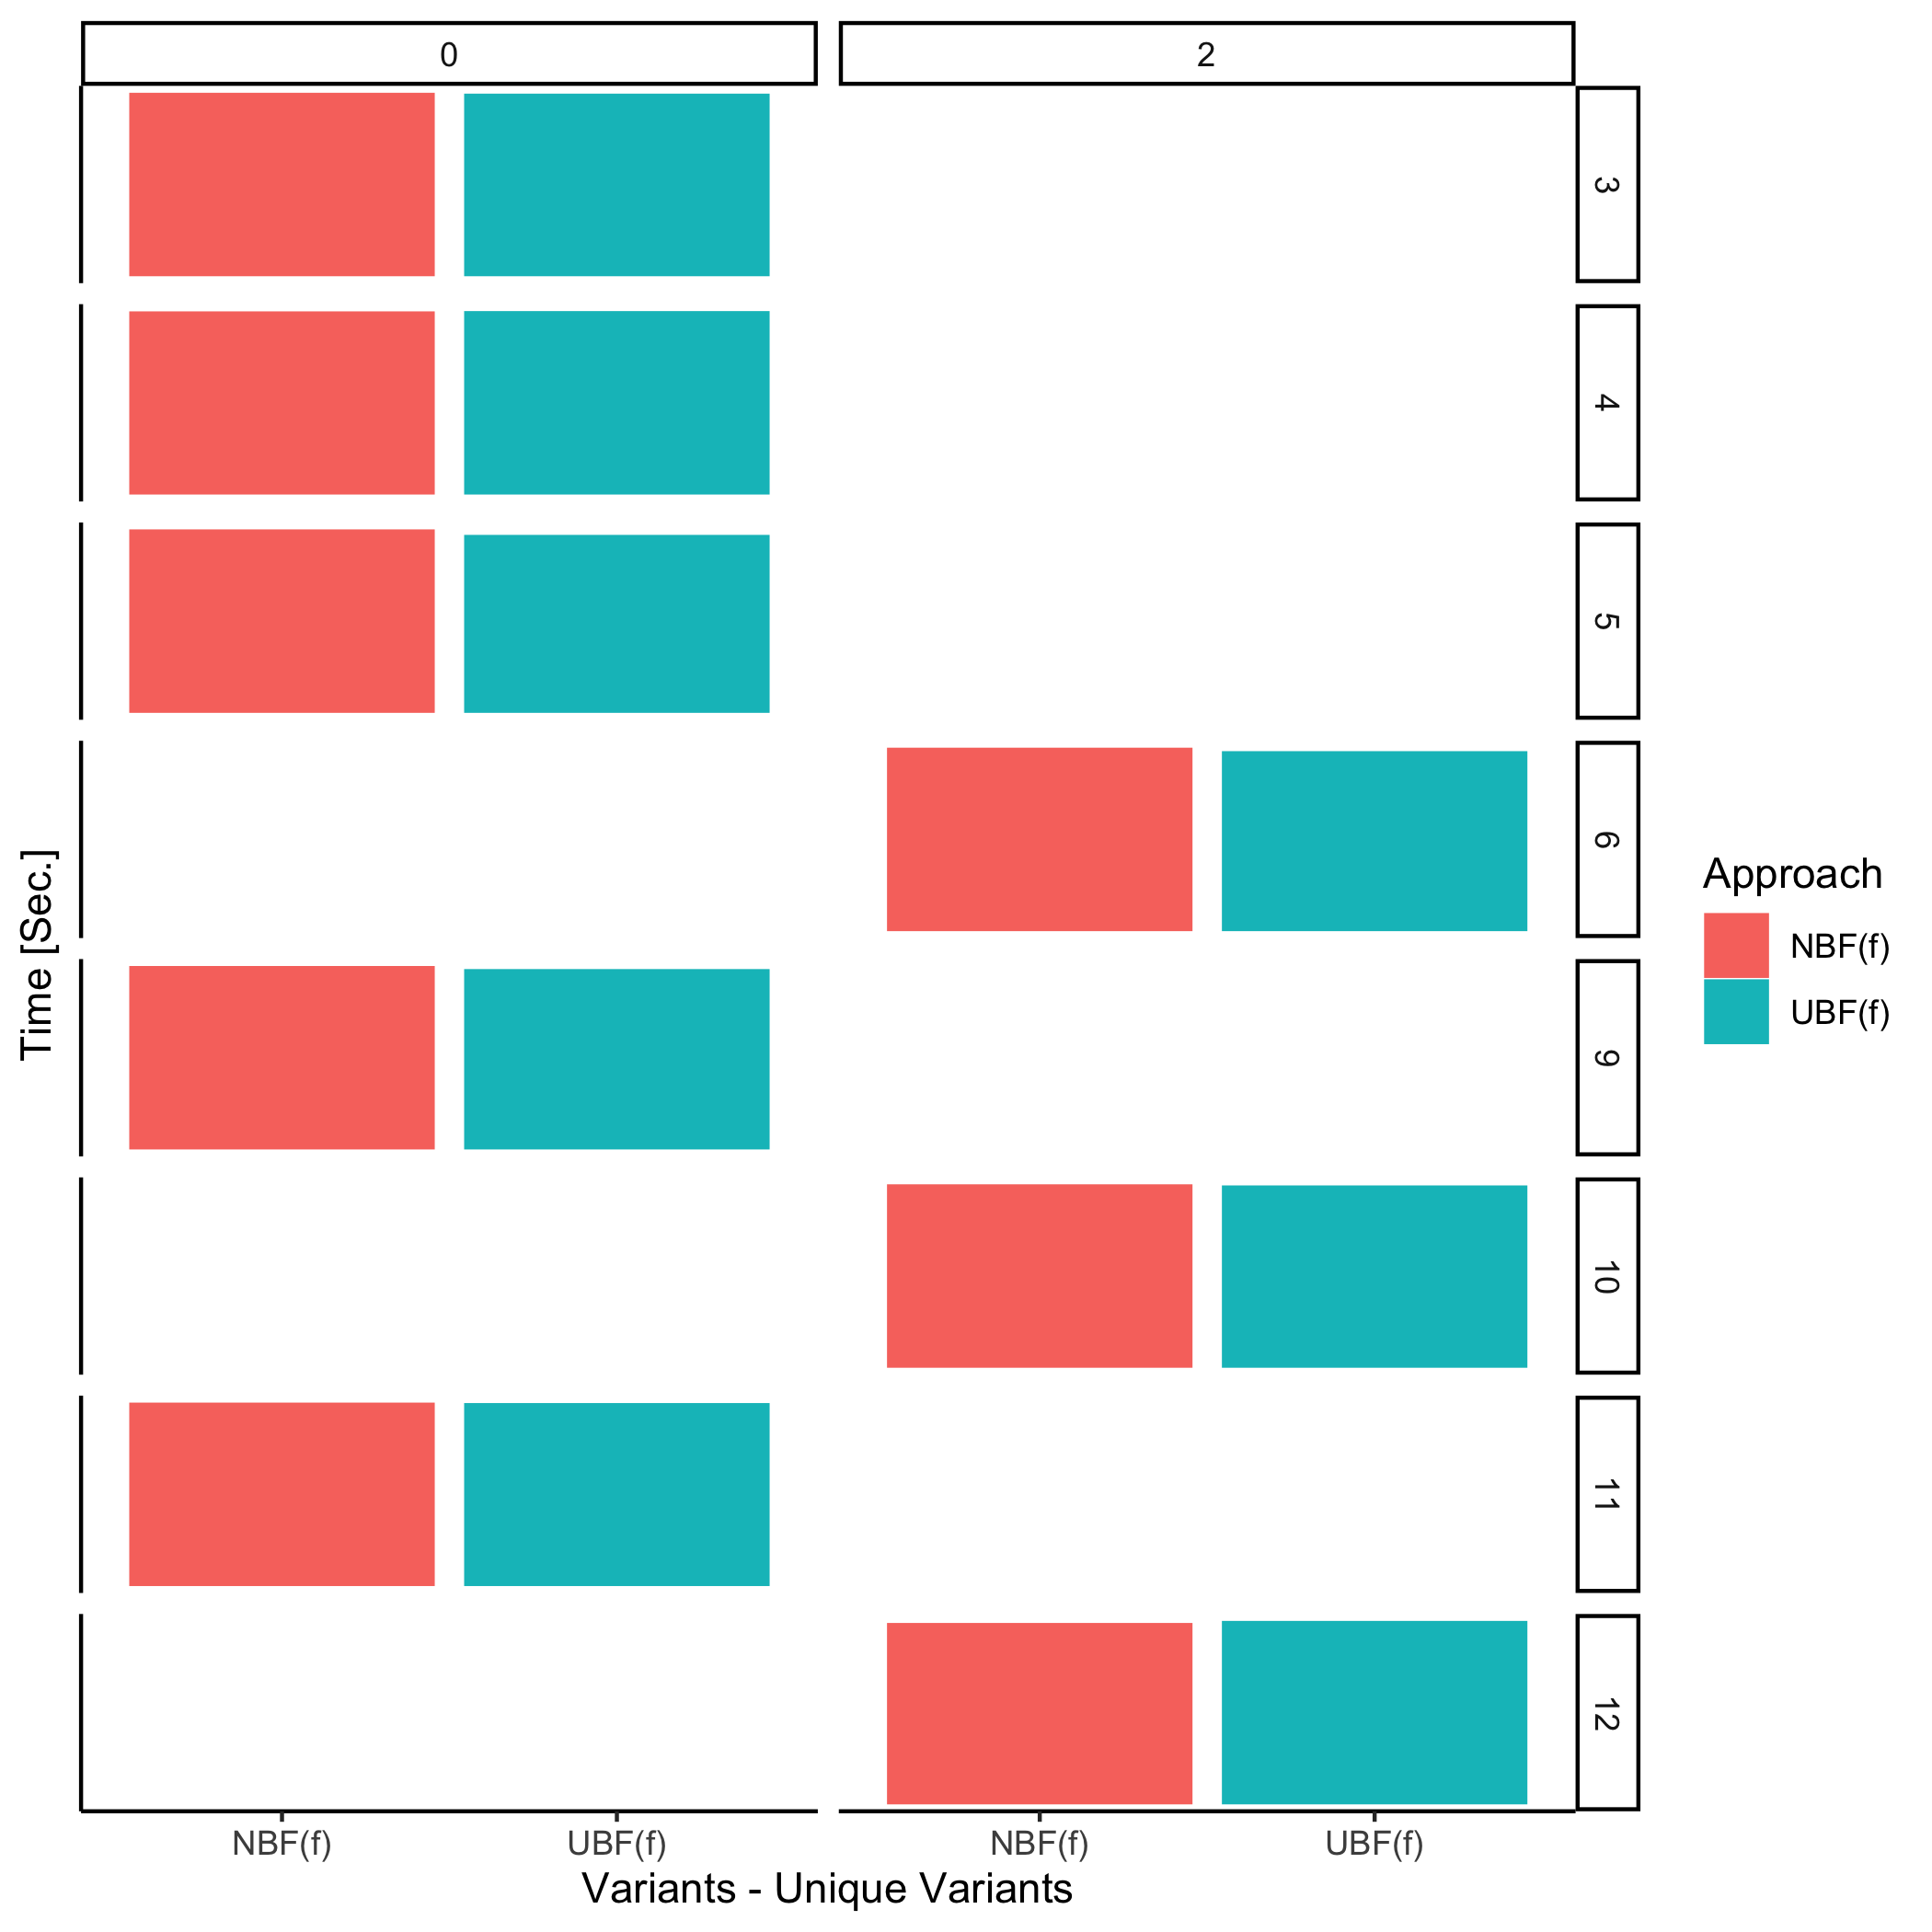
\includegraphics[width=.7\textwidth]{figs/plots/emp-nbff-ubff.png}
\caption[Comparison of the \nbff\ and \ubff\ approaches]{Comparison of the \nbff\ and \ubff\ approaches.}
\label{fig:emp-ubff-ubff}
\end{subfigure}
\begin{subfigure}{0.5\linewidth}
\centering
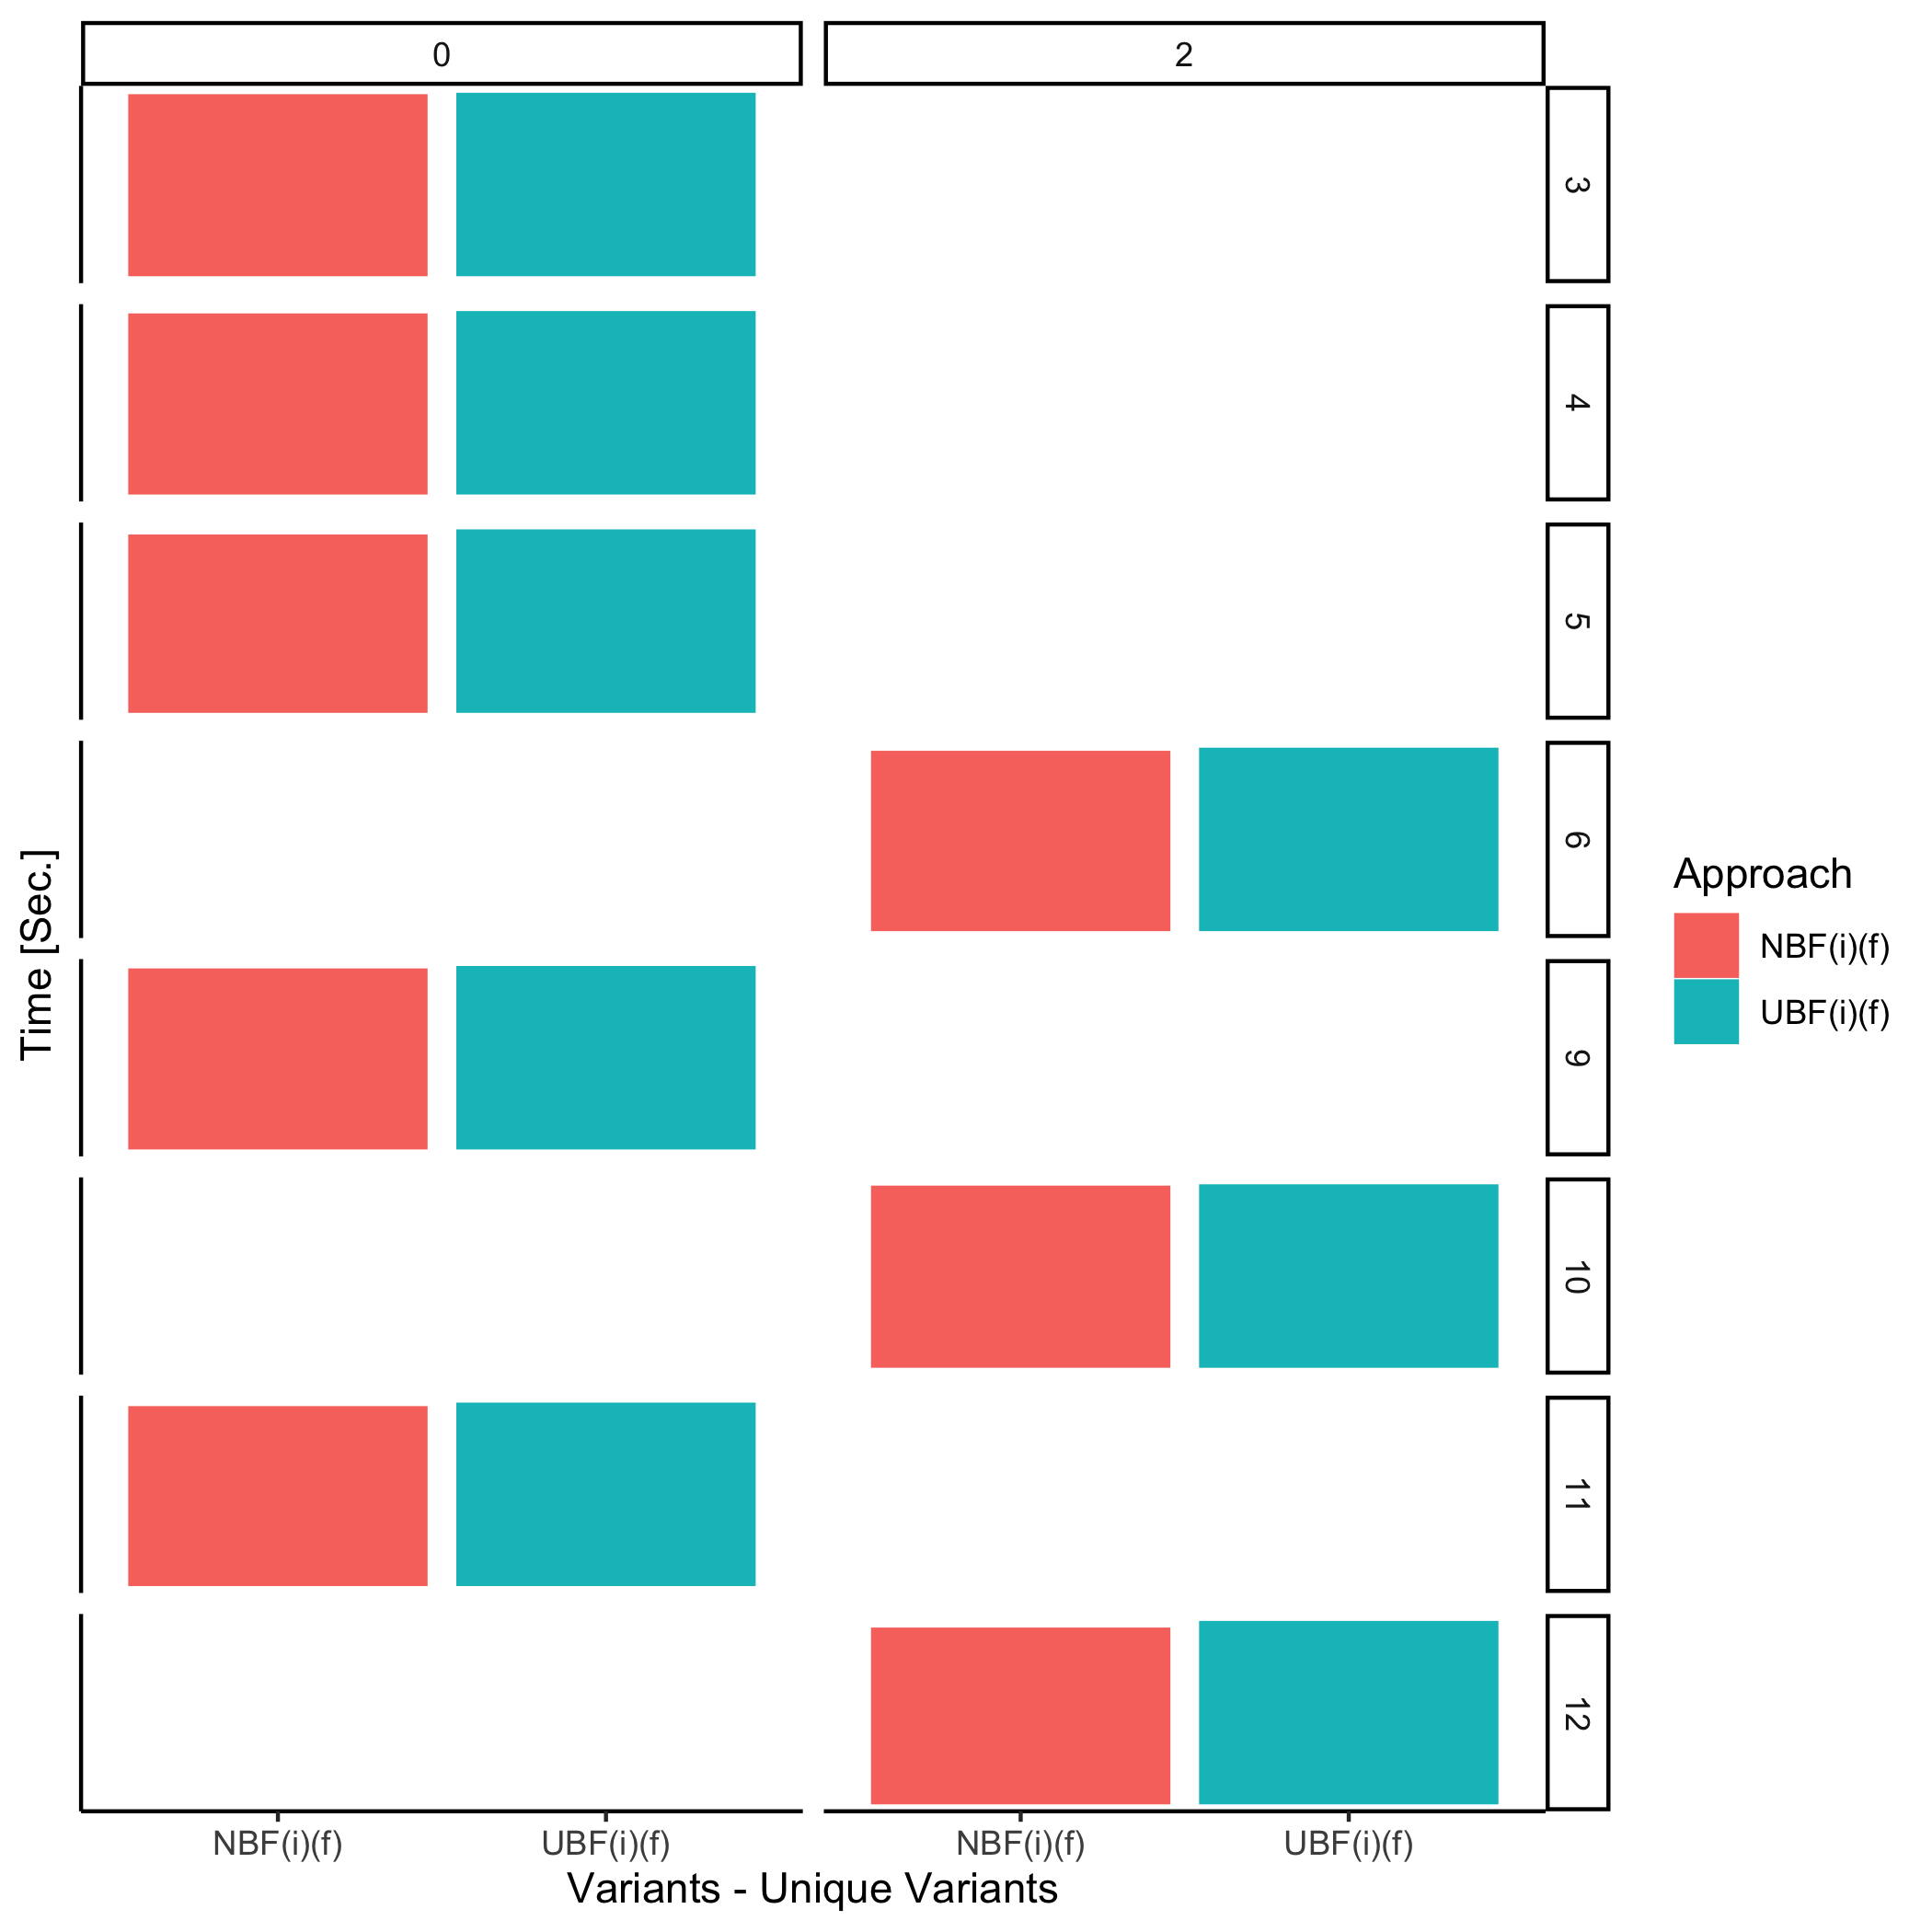
\includegraphics[width=.7\textwidth]{figs/plots/emp-nbfif-ubfif.png}
\caption[Comparison of the \nbfif\ and \ubfif\ approaches]{Comparison of the \nbfif\ and \ubfif\ approaches.}
\label{fig:emp-nbfif-ubfif}
\end{subfigure}
\caption[The effect of the difference of the number of variants and number of unique variants on
the employee VDB]{The effect of the difference of the number of variants and number of unique 
variants on the employee VDB. The categorical boxes on top and the left side of the plots illustrate
the number of variants minus the number of unique variants and the number of queries, respectively.}
\label{fig:emp-vars-minus}
\end{figure}

We now explore the effect of the number of unique variants of queries compared to the
number of variants. This difference would only affect the performance of two groups of 
approaches: 1) \nbf\ vs. \ubf\ and 2) \nbfi\ vs. \ubfi. 
%
Remember that while \nbf\ and \nbfi\ naively process all variants of a variational query
\ubf\ and \ubfi\ only process unique variants of a variational query. That is, the latter approaches
do not unnecessarily repeat a query. This would not make much difference for empty queries, however,
we hypothesize that it significantly affects the performance of \nbf\ and \nbfi\ for non-empty queries. 
%
We explore this hypothesis by the plots shown in \figref{emp-vars-minus} and \figref{enron-vars-minus}.
In these plots, the categorical boxes on top and the left side of the plots indicate
the number of variants minus the number of unique variants and the number/name of queries, respectively.
%
Unfortunately, \figref{emp-vars-minus} does not provide us with much insight. We explore why this 
is the case in \secref{exp-tuples}. However, \figref{enron-vars-minus} confirms our hypothesis that
as the number of differences between the number of variants and unique variants increases, the 
performance of \nbf\ and \nbfi\ decreases compared to \ubf\ and \ubfi. This is due to repeatedly
running an SQL query in addition to the cost of building the variational table for more relational 
tables. 
%
Notice that \figref{enron-vars-minus} does not contain plots comparing approaches that filter out
tuples with unsatisfiable presence conditions whereas \figref{emp-vars-minus}  does. 
We also explain the lack of these plots in \secref{exp-tuples}.


\begin{figure*}[!t]
    \centering
    \begin{subfigure}[t]{0.5\textwidth}
        \centering
        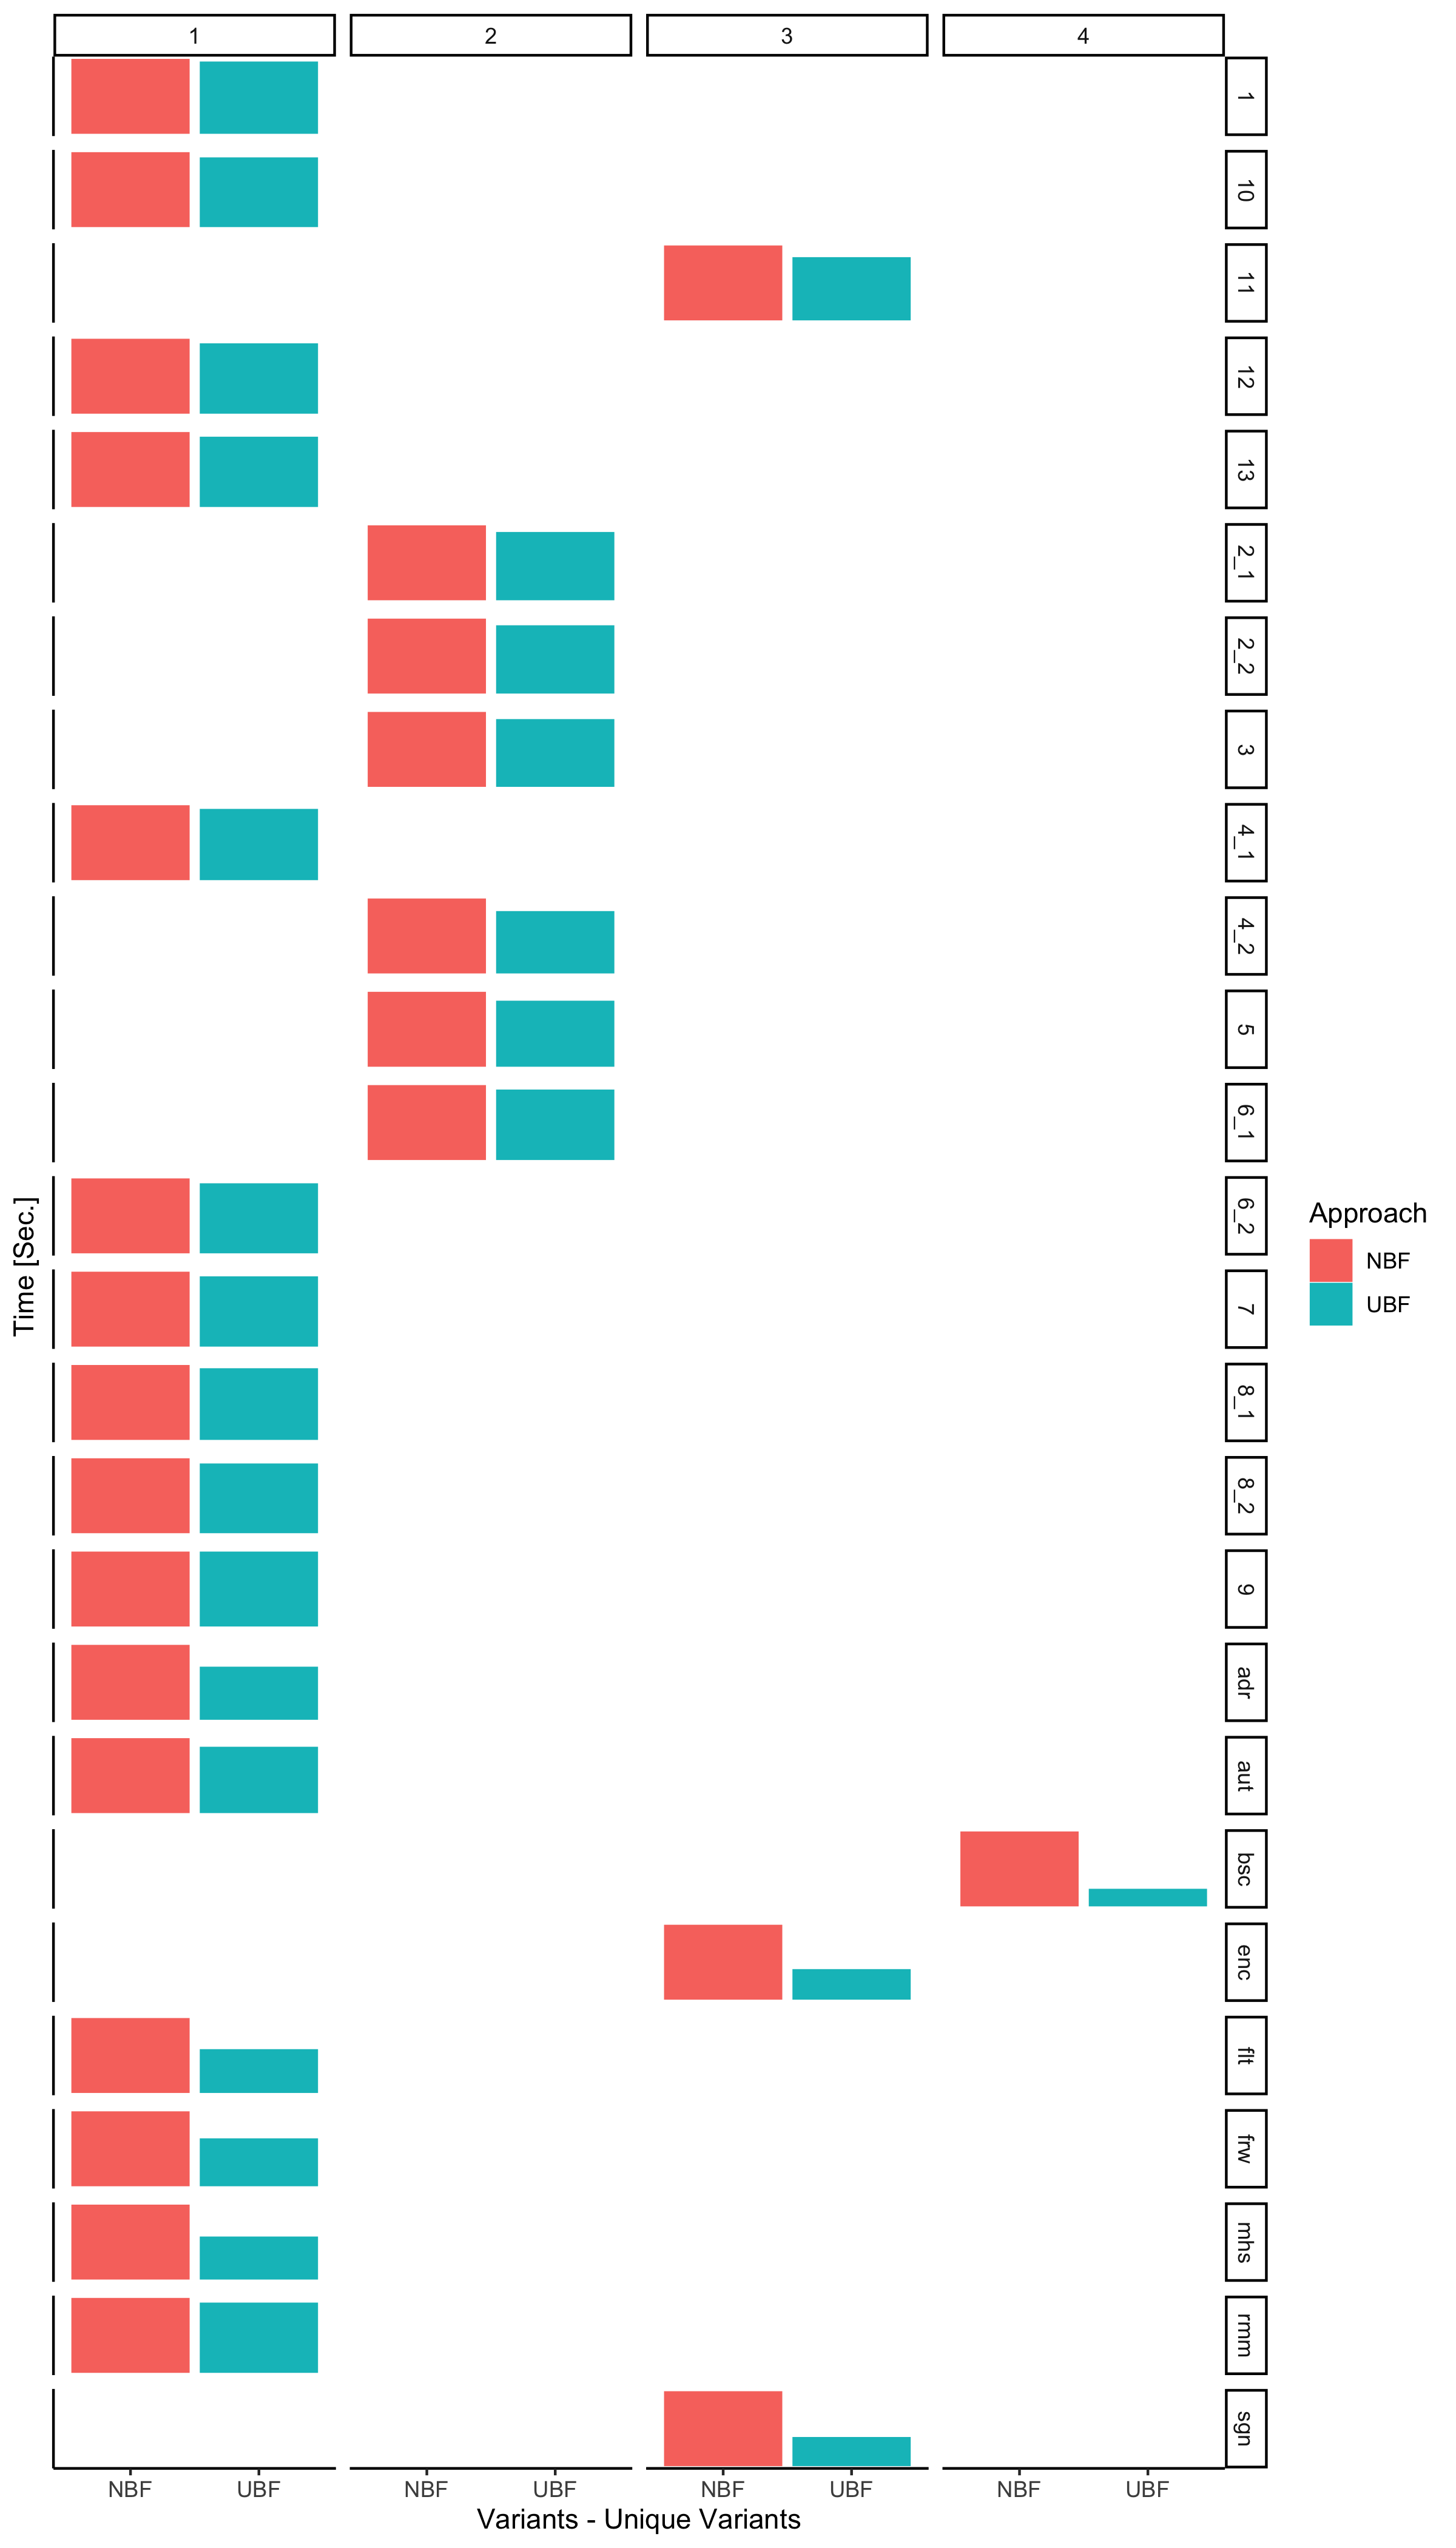
\includegraphics[scale=0.09]{figs/plots/enron-nbf-ubf.png}
        \caption[Comparison of the \nbf\ and \ubf\ approaches]{Comparison of the \nbf\ and \ubf\ approaches.}
        \label{fig:enron-nbf-ubf}
    \end{subfigure}%
    ~ 
    \begin{subfigure}[t]{0.5\textwidth}
        \centering
        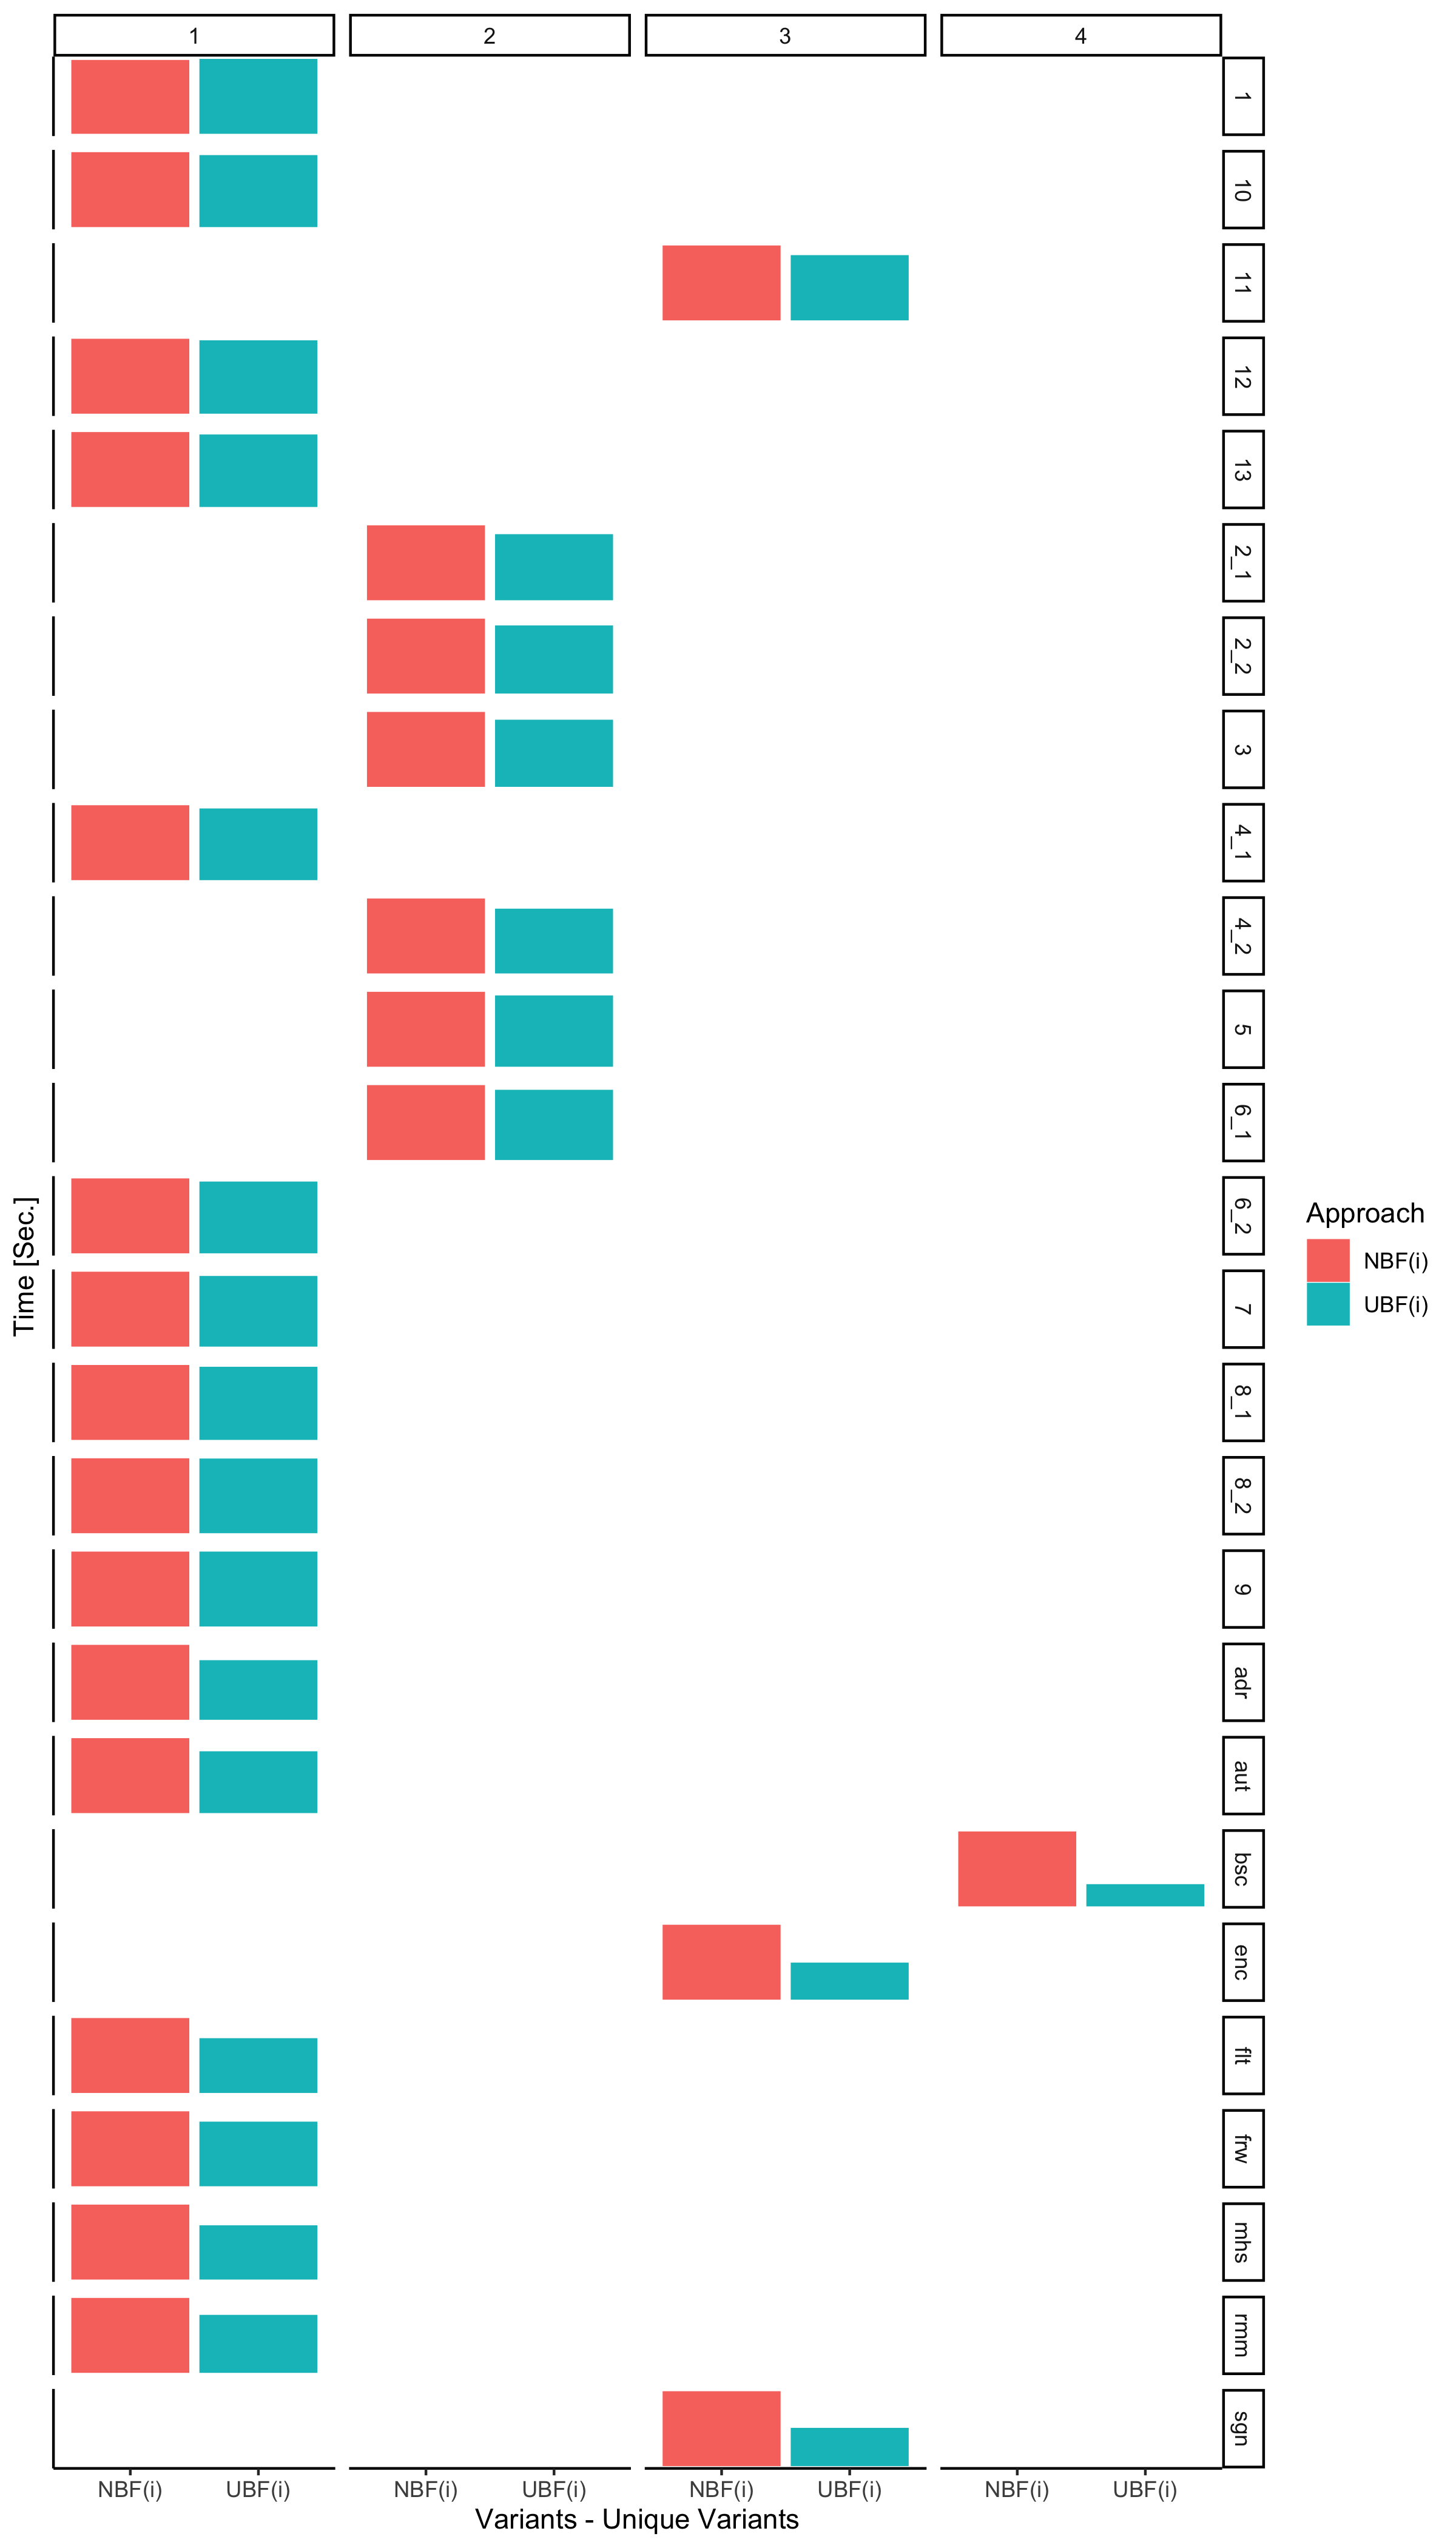
\includegraphics[scale=0.09]{figs/plots/enron-nbfi-ubfi.png}
        \caption[Comparison of the \nbfi\ and \ubfi\ approaches]{Comparison of the \nbfi\ and \ubfi\ approaches.}
        \label{fig:enron-nbfi-ubfi}
    \end{subfigure}
    \caption[The effect of the difference of the number of variants and number of unique variants on
the email VDB]{The effect of the difference of the number of variants and number of unique 
variants on the email VDB. The categorical boxes on top and the left side of the plots indicate
the number of variants minus the number of unique variants and the number/name of queries, respectively.}
\label{fig:enron-vars-minus}
\end{figure*}

